\chapter{Efficient edge-based zonotope vertex enumeration}
\label{chapter:2}
\usection{Introduction}

In this thesis, \emph{in silico} force feasible sets are modeled as a geometric construction based on muscle tension feasible sets, which model the exertable tensions by muscles in a given posture. Their formal definition, when considering forces exerted at the end-effector, is as follows: for $\mathcal{T}\subset \IR^m$, the set of all exertable tensions by m muscles, the force feasible set F⊂R3 at the end effector of an n degrees-of-freedom kinematic chain is defined as:
\begin{align*}
    \mathcal{F} = \left{\mathbf{f}\in\IR^3\mid \exists \mathbf{t}\in \mathcal{T},\quad J^T\mathbf{f} = -L^T\mathbf{t} - \mathbf{G}\right}
\end{align*}
where $J^T\in \mathbb{R}^{n\times 3}$ is the projection of the end-effector Cartesian forces onto the torque space, $L^T\in \IRnm$ is the projection of muscle tensions onto the torque space, and $\mathbf{G}\in\IRn$ is the gravity torque vector.

The reconstruction process occurs \emph{in silico}. Viewed as an optimization process, we compute force feasible sets of a musculoskeletal model in various postures and compare them with reference ones. If some musculoskeletal parameters minimize a metric between \emph{in silico} and experimental force feasible sets, then it can be assumed that the reconstruction succeeded for the given postures and the given metric. Similarly, we can apply the reconstruction process to the \emph{torque feasible set}, corresponding to the set
\begin{align*}
    \left{\tau \in \IR^n \mid \exists \mathbf{t}\in\mathcal{T}, \quad \tau = -L^T\mathbf{t} - \mathbf{G}\right}
\end{align*}

In any case, we suppose the tension set $\mathcal{T}$ to be convex, inducing the force and torque feasible sets to share this property. Consequently, the metric used for comparison should be able to match their surfaces. There remains to compute the surface, which depends greatly on the shape of $\mathcal{T}$.

In this chapter, it will be assumed that $\mathcal{T}$ takes the shape of an $m$-orthotope \emph{i.e.} a hyperrectangle in $m$ dimensions, as shown in figures \ref{fig:joint_torque_simple_2D} and \ref{fig:tension_set_orthotope}. 

\begin{figure}[!htb]
    \captionsetup{justification=centering}
    \begin{minipage}{0.39\linewidth}
        \centering
        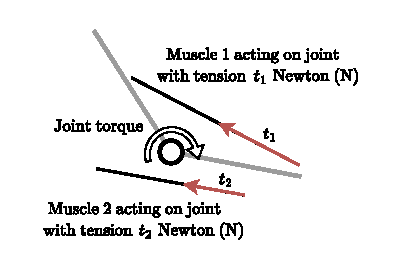
\includegraphics[trim={20 0 20 0}, clip, width=1\linewidth]{img/chapter_2/joint_torque_simple_2D.pdf}
        \caption{Simplified arm with one degree-of-freedom equipped with two muscles described as segments.}
        \label{fig:joint_torque_simple_2D}
    \end{minipage}
    \hfill
    \begin{minipage}{0.59\linewidth}
        \centering
        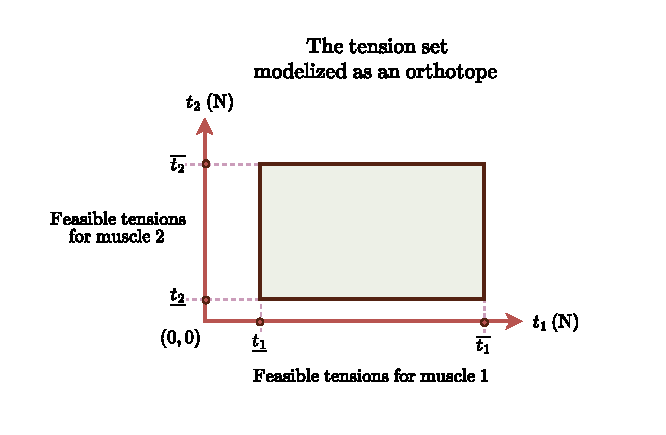
\includegraphics[trim={25 20 40 16}, clip, width=0.98\linewidth]{img/chapter_2/tension_set_orthotope.pdf}
        \caption{A muscle exerts a tension in a feasible range of values. The set of all tension combinations $\mathcal{T}$ is shaped as an orthotope: it assumes muscles act independently from each other.}
        \label{fig:tension_set_orthotope}
    \end{minipage}
\end{figure}

This definition implies the two following statements:
\begin{enumerate}
    \item {For each muscle tension $t_i$ of a muscle $m_i$, there exist positive lower and upper bounds, noted $\underline{t_i}$ and $\overline{t_i}$, defining the feasible tensions exertable by muscle $m_i$. The upper bound corresponds to the feasible muscle tension when it is fully activated, while the lower bound relates to its current passive tension when it is not activated;}
    \item {The shape of an hyperrectangle models how muscles can act together. Essentially, it allows all muscles to exert their maximal tension at the same time.}
\end{enumerate}

The second point is biomechanically a strong assumption. While in a cable robot it could be considered, human muscle activations differ by a neuromotor control whose law is yet to be fully understood. In the context of cable robotics, if cables are considered to be line segments whose feasible tensions are described independently from each other, the tension set $\mathcal{T}$ is shaped as an orthotope. 

Geometrically, when $\mathcal{T}$ is an orthotope, the torque feasible set is a \emph{zonotope} \emph{i.e.} a specific type of polytope described as a projection of a higher-dimensional cube. In the context of computing the vertices of a zonotope, since a $m$-orthotope is the image of a $m$-cube under an invertible affine transformation, we can without loss of generality assimilate $\mathcal{T}$ to the $m$-dimensional cube $[0,1]^m$, as shown in the figure \ref{fig:invertible_transfo_cube_orthotope}. We say that a $m$-orthotope and a $m$-cube are \emph{affinely equivalent}. 
\begin{figure}[!htb]
    \captionsetup{justification=centering}
    \begin{minipage}{1\linewidth}
        \centering
        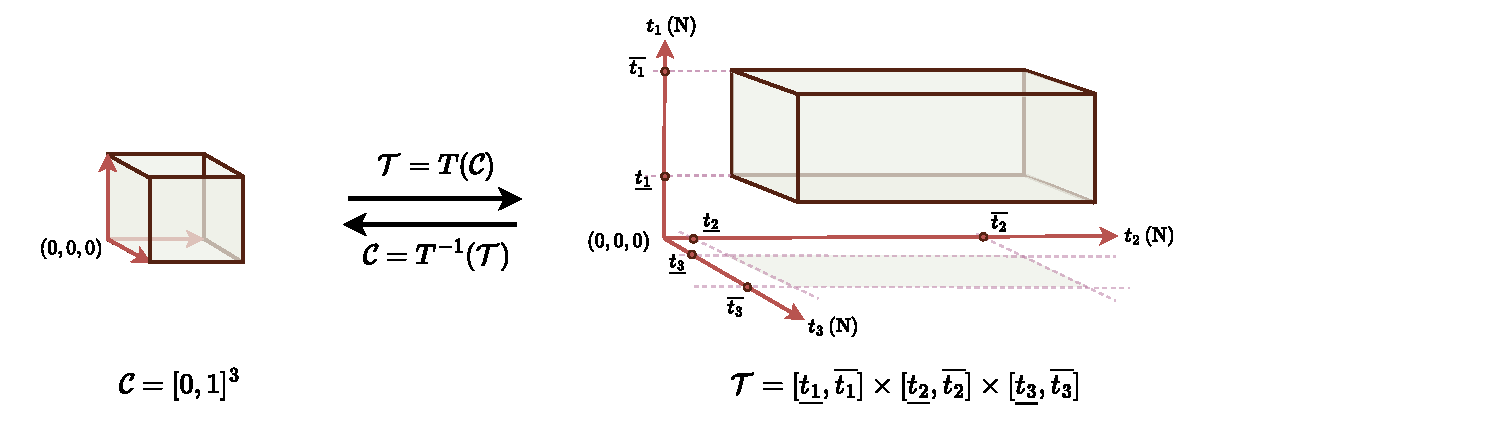
\includegraphics[trim={20 20 150 0}, clip, width=1\linewidth]{img/chapter_2/invertible_transformation.pdf}
        \caption[]{To consider the torque feasible set as a projection of the unit cube $\mathcal{C}=[0,1]^3$, consider the invertible affine transformation $T\,\colon \IR^3 \to \IR^3$ defined as:
        \begin{minipage}{\linewidth}
            \begin{align*}
                T(\mathbf{t}) &= D\mathbf{t} + \underline{\mathbf{t}}, \quad \text{for } D = \begin{pmatrix}
                    \overline{t_1} - \underline{t_1} & 0 & 0 \\
                    0 & \overline{t_2} - \underline{t_2} & 0 \\
                    0 & 0 & \overline{t_3} - \underline{t_3}
                \end{pmatrix} \text{ and } \underline{\mathbf{t}} = \begin{pmatrix}
                    \underline{t_1} \\ \underline{t_2} \\ \underline{t_3}
                \end{pmatrix}
            \end{align*}
        \end{minipage}

        Thus, $\mathcal{T} = T(\mathcal{C})$ and the torque feasible set is described as 
        $\left\{\tau \in \IR^3 \mid -LD\mathbf{t} -L\underline{\mathbf{t}} - \mathbf{G},\quad \mathbf{t}\in\mathcal{C}\right\}$, which is clearly an affine projection of a cube so it is a zonotope by definition.}
        \label{fig:invertible_transfo_cube_orthotope}
    \end{minipage}
\end{figure}

Zonotopes have multiple possible representations including either a non-squared matrix, a set of vertices, delimiting hyperplanes, or even \emph{cells} which characterize the cube vertices whose projections are the zonotope vertices. Several algorithms exist to transit from one representation to another, whose goals are to be efficient in time and space. This chapter offers a new perspective on representing zonotopes using their edges, and describes an algorithm to compute them directly from a matrix representation of a zonotope. To achieve this goal, let's first dive onto zonotope formalism.

Let $\Zono \subset \IRn$ be a $n$-zonotope, \emph{i.e.} 
the Minkowski sum of $n$-dimensional segment vectors $\Zono = \mathbf{c} + \bigoplus_{i=1}^m \alpha_i \mathbf{g}_i$ for $\mathbf{c} \in \IRn$, $\mathbf{g}_i \in \IRn$ for $i=1,\dots,m$ such that all the $\mathbf{g}_i$ span $\IRn$, and $\alpha_i\in[0,1]$. It corresponds to the following set:
\begin{align*}
    \Zono &= \left\{ \mathbf{z} \in \IR^n \mid \mathbf{z} = \mathbf{c} + \sum_{i=1}^m \alpha_i \mathbf{g}_i,\quad \alpha_i \in [0,1],\, \mathbf{c}, \mathbf{g}_1,\cdots,\mathbf{g}_m\in\IR^n \right\} \\
    &= \mathbf{c} + \bigoplus_{i=1}^m \alpha_i \mathbf{g}_i
\end{align*}

The vectors $\mathbf{g}_i$ are called \emph{generators} and are usually concatenated into columns of a matrix $G\in\IRnm$. For consiveness, a zonotope is denoted using directly its translation and its generators as $\Zono(\mathbf{c}, G)$, or $\Zono(G)$ if there is no translation. The notation $\Zono(n, m)$ is also convenient to directly refer to the size of the matrix $G$. It is assumed that generators are non-null and that any combination of $n$ of them span $\IRn$. In this case, the generators are said to be in \emph{general position}.

\begin{figure}[!htb]
    \captionsetup{justification=centering}
    \begin{minipage}{0.49\linewidth}
        \centering
        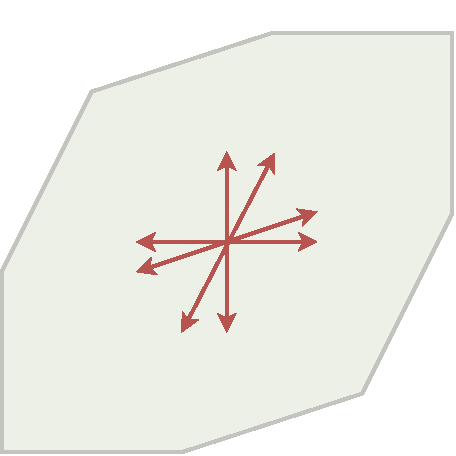
\includegraphics[trim={0 0 0 0},clip, width=0.6\linewidth]{img/chapter_2/zonotope_2d_4g.pdf}
    \end{minipage}
    \hfill
    \begin{minipage}{0.49\linewidth}
        \centering
        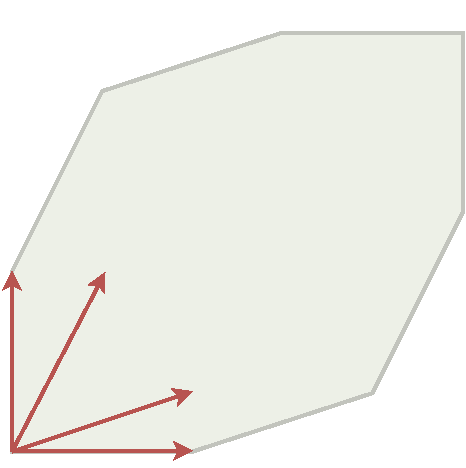
\includegraphics[trim={0 0 0 0},clip,width=0.6\linewidth]{img/chapter_2/zonotope_2d_4g_alt.pdf}
    \end{minipage}
    \caption{Both constructions lead to the same 2D zonotope generated by $4$ generators: the differences lie in the bounds defined for $\alpha_i$, which are $[-1,1]$ for the left zonotope and $[0, 1]$ for the right, and the center $\mathbf{c}$.}
    \label{fig:a_simple_zonotope}
\end{figure}

A zonotope is a specific type of convex polytope, so it can be described via its vertices ($\mathcal{V}$-representation) or a set of inequalities ($\mathcal{H}$-representation), as shown in figure \ref{fig:zonotope_vertices_hyperplanes}. Several zonotope applications can be found as bounding volumes in collision detection (\cite{guibasZonotopesBoundingVolumes},) as bounding disturbances and measurement errors (\cite{scottInputDesignGuaranteed2014}), but also in approximating the domain of a function of several variables (\cite{stinsonRandomizedAlgorithmEnumerating2016}).
More recently in robotics, a neural network was used to predict a path of reachable sets in an environment crowded with dynamic obstacles modelized as zonotopes (\cite{shamsahSociallyAcceptableBipedal2024}).

\begin{figure}[!htb]
    \captionsetup{justification=centering}
    \begin{minipage}{0.49\linewidth}
        \centering
        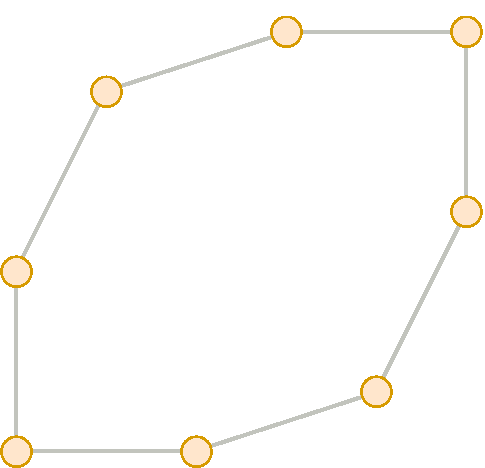
\includegraphics[trim={0 0 0 0},clip, width=0.6\linewidth]{img/chapter_2/zonotope_vertices.pdf}
    \end{minipage}
    \hfill
    \begin{minipage}{0.49\linewidth}
        \centering
        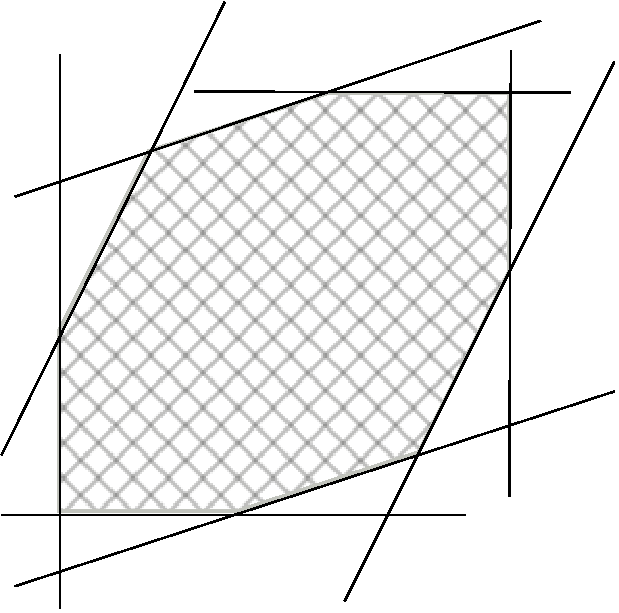
\includegraphics[trim={0 0 0 0},clip,width=0.75\linewidth]{img/chapter_2/zonotope_hyperplanes.pdf}
    \end{minipage}
    \caption{Any zonotope can be represented by either a set of vertices or bounding hyperplanes. Using vertices, a zonotope corresponds to the convex hull of these vertices (all interior and surface points). For bounding hyperplanes, these constraint the locations of zonotope's points within a region of the space so that the direction of the halfspace must be precised for each hyperplane.}
    \label{fig:zonotope_vertices_hyperplanes}
\end{figure}

The process of retrieving zonotope vertices from its description using generators is a combinatorial problem described as the \emph{vertex enumeration problem}. The explicit enumeration of zonotope vertices is required for instance in the fixed rank integer quadratic program (\cite{ferrezSolvingFixedRank2005a}), in signal processing (\cite{markopoulosOptimalAlgorithmsL_12014}) and in linear regression models with interval data (\cite{cernyPossibilisticApproachLinear2013}).

Unfortunately, converting zonotope generators to vertices or bounding hyperplanes is a combinatorial problem. As the dimension or the number of generators increases, the number of vertices does too: theorem 3.1 from (\cite{ferrezSolvingFixedRank2005a}) recalls that the number of vertices of a $n$-zonotope $\mathcal{Z}$ with $m$ generators is $\leq 2 \sum_{i=0}^{n-1} \binom{m-1}{i}$, with equality satisfied when the generators are in general position. For instance, a 3D zonotope can have up to $92$ vertices if it is defined by $10$ generators; $2452$ if it has $50$ generators; and $9902$ vertices for $100$ generators. Similarly, for a $n$-zonotope with $50$ generators, it has up to $39300$ vertices for $n=4$, more than $5.6\times 10^{14}$ for $n=25$ and more than $1.1\times 10^{15}$ for $n=50$. In a biomechanical context, by considering the Stanford's upper limb musculoskeletal model consisting of $50$ muscles and $7$ degrees-of-freedom (\cite{holzbaurModelUpperExtremity2005}), the torque feasible set has at most $32244452$ vertices. Consequently, the required space to describe all the vertices becomes large very quickly, independently of the efficiency of an algorithm enumerating them. 

The following section \ref{edge_enumeration_algorithm_section} presents a novel efficient zonotope edge enumeration algorithm, called \emph{EdgeEnum} which can be used to enumerate vertices of a zonotope. Section \ref{time_complexity_edgeenum} shows that EdgeEnum is indeed theoretically \emph{efficient} by proving the polynomiality of both its time and space complexity when $n$ is fixed. An asymptotic growth comparison is also performed over various recent enumeration algorithms adapted to the zonotope vertex enumeration problem. Section \ref{time_benchmark} compares the time benchmark of multiple algorithms to show that in practice EdgeEnum is faster for zonotopes described by $m\geq 10$ generators in dimensions $n\geq 6$. Section \ref{sec:approximation_of_vertices_zonotope} offers some insights on time computation of approximated vertex enumeration algorithms, in order to show that in our context, the current computation times are not fast enough, whether using approximated or exact algorithms. Finally, section \ref{conclusion_zonotope_enum_algorithm} summarizes the results and advantages offered by our approach, such as the easyness of implementation and the possible parallelism in comparison to existing methods, while bringing some light upon the effectiveness of using vertices to describe zonotope characteristics of interest such as its global shape and orientation.

\section{The edge enumeration algorithm}
\label{edge_enumeration_algorithm_section}

While enumerating zonotope vertices is the main goal, we shall present an algorithm which enumerate its edges, then describe an edges-to-vertices conversion algorithm which is negligeable in additional computation time. The edge enumeration algorithm takes as input the generator matrix of a $n$-zonotope $\Zono$ with $m$ generators in general position and returns a set of $m$-cube edges which map to the edges of $\Zono$.

Vertices \emph{do not} contain information about other vertices, whereas edges are linked to at least $2$ vertices, so that the knowledge of an edge allows us to describe its extremal vertices. Our novel approach use this information in order to make vertex enumeration faster, by enumerating zonotope edges. Since a zonotope is the projection of a higher-dimensional cube, its edges are also the projection of some cube edges, so constructing edges of the cube in higher dimension is required.

\subsubsection*{From cube edges to zonotope edges}

The construction of the edges of a $m$-dimensional hypercube, also called a $m$-cube, is an iterative process over dimensions $2$ to $m$ (cf. figure \ref{fig:cube_edge_construction}). Starting from a square (or the $2$-cube), each of its edges are embedded in 3D then duplicated and translated by $1$ along the newly created dimension. Once done, there remains to create new edges arising from the duplication: for each vertex $v$ in the previous step, a segment is created between $v$ and its newly duplicated and translated version $v'$. The process is then iterated until the $m^{\text{th}}$ dimension is reached: all of the $m$-cube edges are enumerated.

\begin{figure}[!htb]
    \captionsetup{justification=centering}
    \centering
    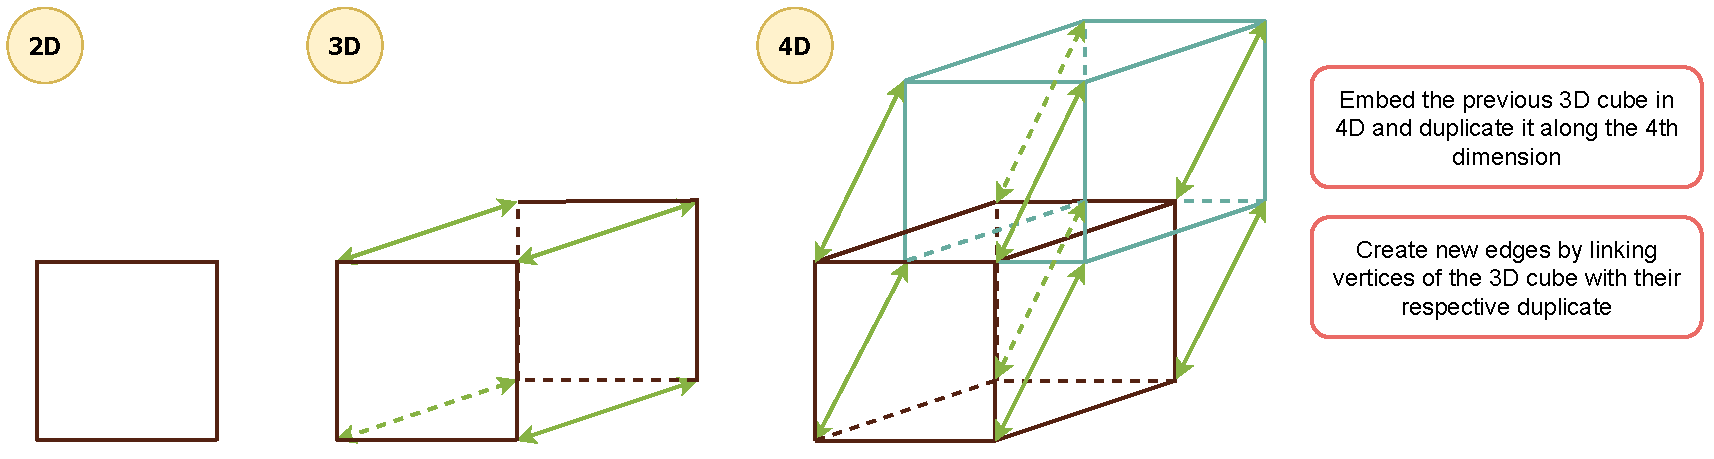
\includegraphics[trim={0 0 0 0},clip, width=1.0\linewidth]{img/chapter_2/zonotope_construction_from_cube_edge_duplication.pdf}
    \caption{Constructing the edges of a zonotope with $4$ generators requires constructing the edges of a $4$-dimensional hypercube. The process is iterative and starts from the square to retrieve the cube, then the $4$-cube. The creation of new edges arising at each new step correspond to the green double arrows.}
    \label{fig:cube_edge_construction}
\end{figure}


Once all $m$-cube edges are enumerated, projecting them via the generator matrix of the considered zonotope gives us something similar to the figure \ref{fig:from_cube_edges_to_zonotope_edges}: a bunch of segments which seems to encapsulate the zonotope.

\begin{figure}[!htb]
    \captionsetup{justification=centering}
    \centering
    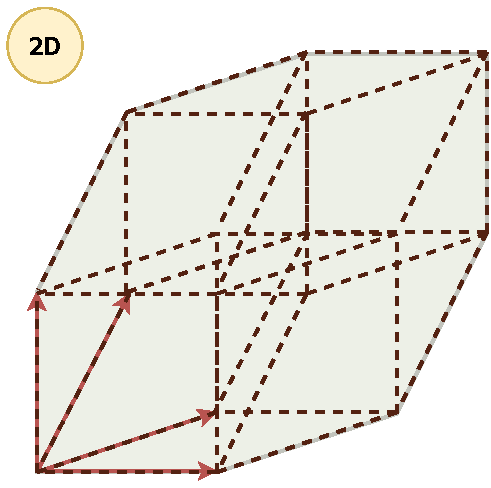
\includegraphics[trim={0 0 0 0},clip, width=0.3\linewidth]{img/chapter_2/zonotope_after_cube_duplication.pdf}
    \caption{Projecting the $4$-cube edges via the generator matrix of a 2D zonotope with $4$ generators.}
    \label{fig:from_cube_edges_to_zonotope_edges}
\end{figure}

This phenomenon is due to a parallelism property specific to zonotopes. Two segments or lines are \emph{parallel} if their direction vectors are colinear.

\begin{lemmabox}{Parallelism of zonotope edges with the generators}{zono_edges_parallel}
    For any $n$-dimensional zonotope $\Zono \subset \IRn$ with $m$ generators, then each of its edge is parallel to one of its generator.

    Moreover, each projected edge of the $m$-cube is also parallel to one of the generators.
\end{lemmabox}
\begin{proof}
A linear or affine map preserves parallelism. 
Consider a zonotope $\Zono$ described by generators $\mathbf{g}_1,\dots,\mathbf{g}_m \in \IRn$ in general position. Denote by $G$ the generator matrix. If $n\geq 2$, then edges of the $m$-cube surject onto the zonotope edges clearly.
Since edges of the $m$-cube can be grouped by parallelism by a representing vector $\mathbf{r}_i = e_i \in \IRm$ where $e_i$ corresponds to the $i^{\text{th}}$ vector of the canonical basis of $\IRm$, we have that $G\mathbf{r}_i = \mathbf{g}_i$. This ensures that when an edge cube is projected via $G$, it necessarily will be parallel to one of the generator.
\end{proof}

\begin{figure}[!htb]
    \captionsetup{justification=centering}
    \begin{minipage}{0.49\linewidth}
        \centering
        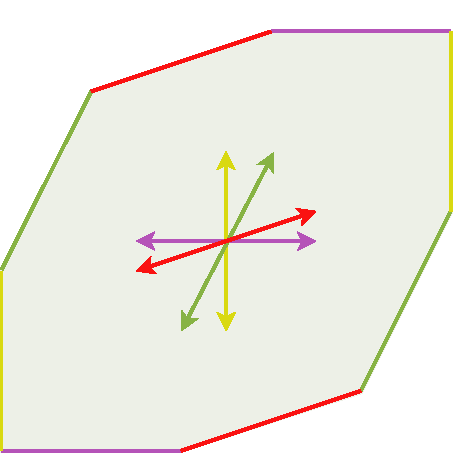
\includegraphics[trim={0 0 0 0},clip, width=0.55\linewidth]{img/chapter_2/zonotope_edges_parallel_generator.pdf}
    \end{minipage}
    \hfill
    \begin{minipage}{0.49\linewidth}
        \centering
        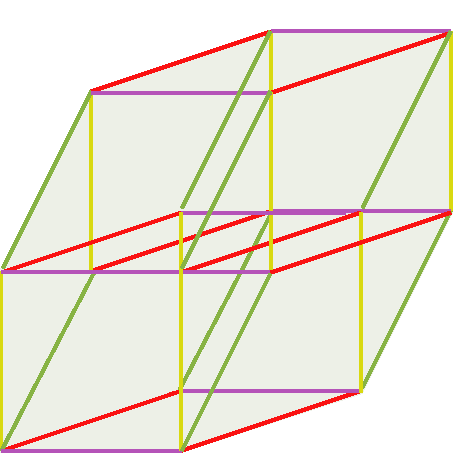
\includegraphics[trim={0 0 0 0},clip,width=0.55\linewidth]{img/chapter_2/zonotope_edges_parallel_generator_alt.pdf}
    \end{minipage}
    \caption{To the left: each edge of a zonotope $\Zono$ is parallel to one of its generator. To the right: projecting a $4$-cube edge via the generator matrix of $\Zono$ produces a line segment parallel to one of the generator.}
    \label{fig:zonotope_edges_parallel}
\end{figure}

% Results about cube edges projected are not new, and enumerating all of them is actually computationally very demanding, as the number of edges of the $m$-cube is much bigger than the number of its vertices. 
Unfortunately, for a zonotope $\Zono(\mathbf{c}, G)$, we could not enumerate each edge $\mathbf{e}$ of an $m$-cube and project them via $\mathbf{e} \mapsto \mathbf{c} + G\mathbf{e}$ to obtain the zonotope edges, due to the high combinatorics involved in the number of possible edges. This amounts to $m2^{m-1}$ edges for a $m$-cube, which is greater than $2^m$, the amount of vertices and would make our approach worse than the naive algorithm.

Our novel approach uses a straight-forward elimination technique to remove useless cube edges as described in the following paragraphs.


\subsubsection*{The convex hull of parallel lines}
As seen in lemma \ref{th:zono_edges_parallel}, in a zonotope each edge is parallel to one of the generator. More than that: each edge of the $m$-cube will map to a segment parallel to a generator. This means that it is possible to \emph{group} the projected cube edges by parallelness; the group representant being one of the generator. For each group, the extremal segments define the edges of the zonotope parallel to the considered generator.
Suppose we group these projected edges by parallelism. The next question is: \emph{how do I select only the ones on the zonotope surface?} While it is a very difficult question to answer for a set consisting of various segments, we are working with projected edges which are all parallel to a generator so that this difficulty is leveraged. 

We shall call the process of retrieving extremal edges as the \emph{convex hull of parallel lines}. Usually and in practice, convex hulls are implemented for sets of points. In this specific case of parallelism, we shall establish an algorithm which selects extremal edges by modifiying the problem as a classic convex hull of a set of points.

Let us introduce it by a 2D example which will generalize well for any dimension: proceeding step by step, consider the first iteration of the algorithm. Edges of a square are created, then they are embedded in 3D and projected via the submatrix of $G$ consisting of the two first columns. This gives three group of edges as shown by the edge colours in figure \ref{fig:convex_hull_lines_intro}.
\begin{figure}[!htb]
    \captionsetup{justification=centering}
    
    \centering
    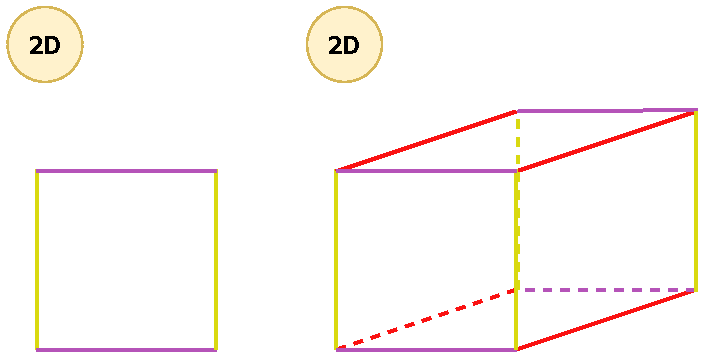
\includegraphics[trim={0 0 0 0},clip,width=0.5\linewidth]{img/chapter_2/zonotope_convex_hull_lines_intro.pdf}

    \caption{The edges on the right are created from embedding and duplicating the square edges to create a cube, then are projected onto the plane via the two first columns of $G$.}
    \label{fig:convex_hull_lines_intro}
\end{figure}

Now, consider a group of parallel edges, the purple ones. We shall consider them as lines. Then, an arbitrary point in the zonotope space is selected and is projected orthogonally onto each line. At any step of the algorithm, these projected points span at most a $n-1$-dimensional space if the zonotope is of dimension $n$. The convex hull operation is thus applied on this set of projected points and only the edges associated to points on the convex hull are kept for the next iteration (cf. figure \ref{fig:convex_hull_lines}).
\begin{figure}[!htb]
    \captionsetup{justification=centering}
    
    \centering
    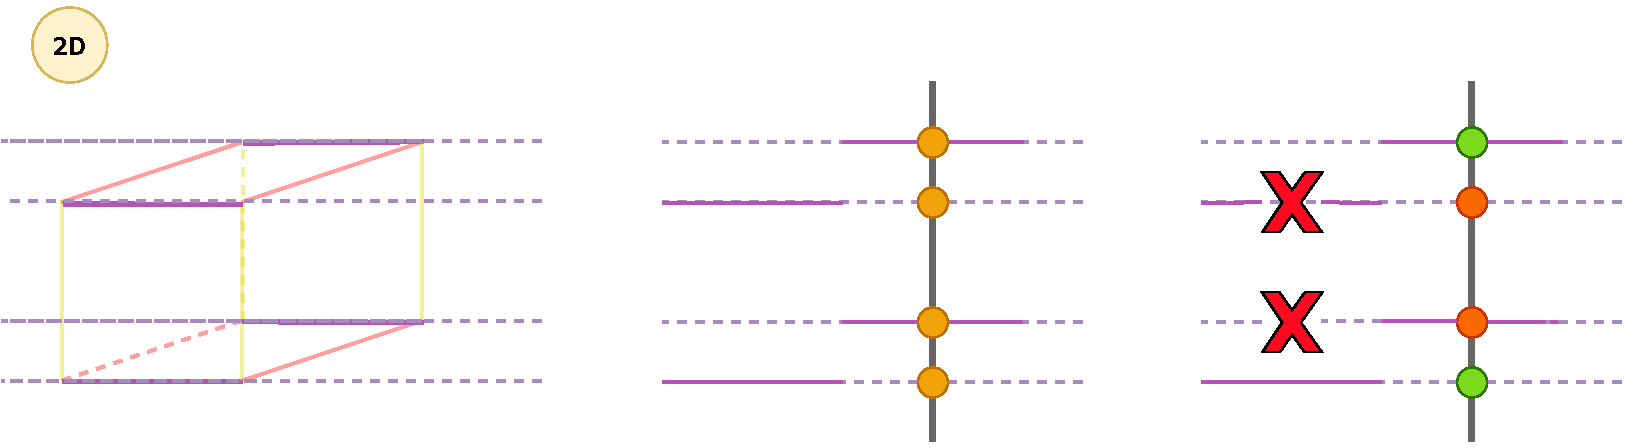
\includegraphics[trim={0 0 0 0},clip,width=1\linewidth]{img/chapter_2/zonotope_convex_hull_lines.pdf}

    \caption{From left to right: select a group of parallel edges and consider them as lines. Then project an arbitrary point orthogonally onto these lines. Finally, apply the convex hull operation onto these points to retrieve the extremal associated edges. This works in any dimension, as long as a set of parallel lines is considered.}
    \label{fig:convex_hull_lines}
\end{figure}

We shall repeat this process for all group of edges, which amounts to the number of dimensions the underlying cube is defined as, as shown in figure \ref{fig:convex_hull_lines_repeat_groups}.

\begin{figure}[!htb]
    \captionsetup{justification=centering}
    
    \centering
    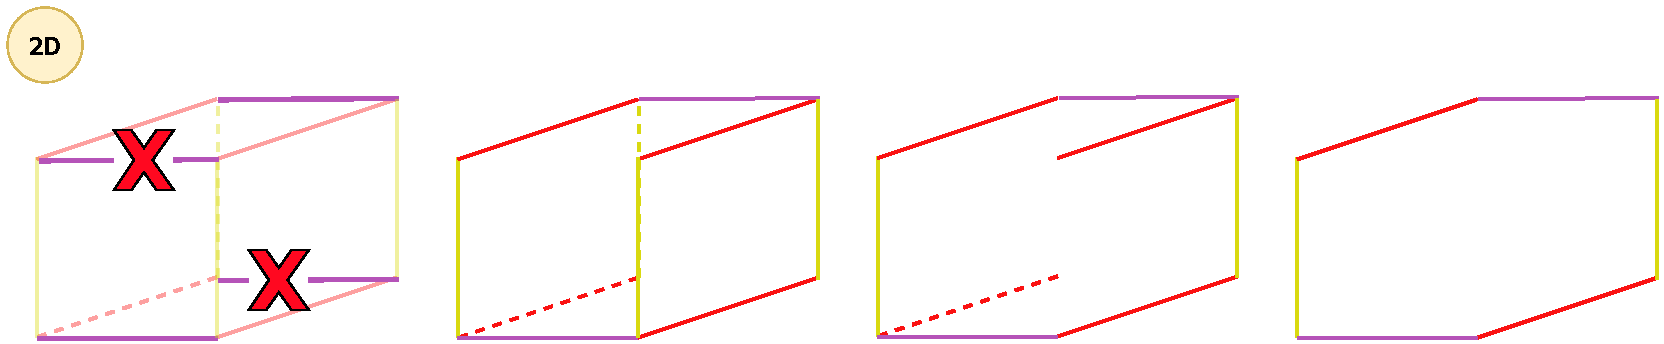
\includegraphics[trim={0 0 0 0},clip,width=1\linewidth]{img/chapter_2/zonotope_edge_elimination_repeat.pdf}

    \caption{Selection of the extremal edges for each group of parallel edges by applying the convex hull of parallel lines. First purple edges, then yellow ones and finally red ones.}
    \label{fig:convex_hull_lines_repeat_groups}
\end{figure}

Once all groups have been treated, we are left with only the necessary edges required to produce the edges of the zonotope generated by the three first columns of $G$. We shall proceed to the embedding, duplication and translation process to create the new edges in $4D$, and project them in this time via the submatrix of $G$ consisting of the four first columns. The algorithm stops when after multiple iterations, the selected cube edges are from the $m$-cube (cf. figure \ref{fig:zonotope_edges_elimination_end}).
\begin{figure}[!htb]
    \captionsetup{justification=centering}
    
    \centering
    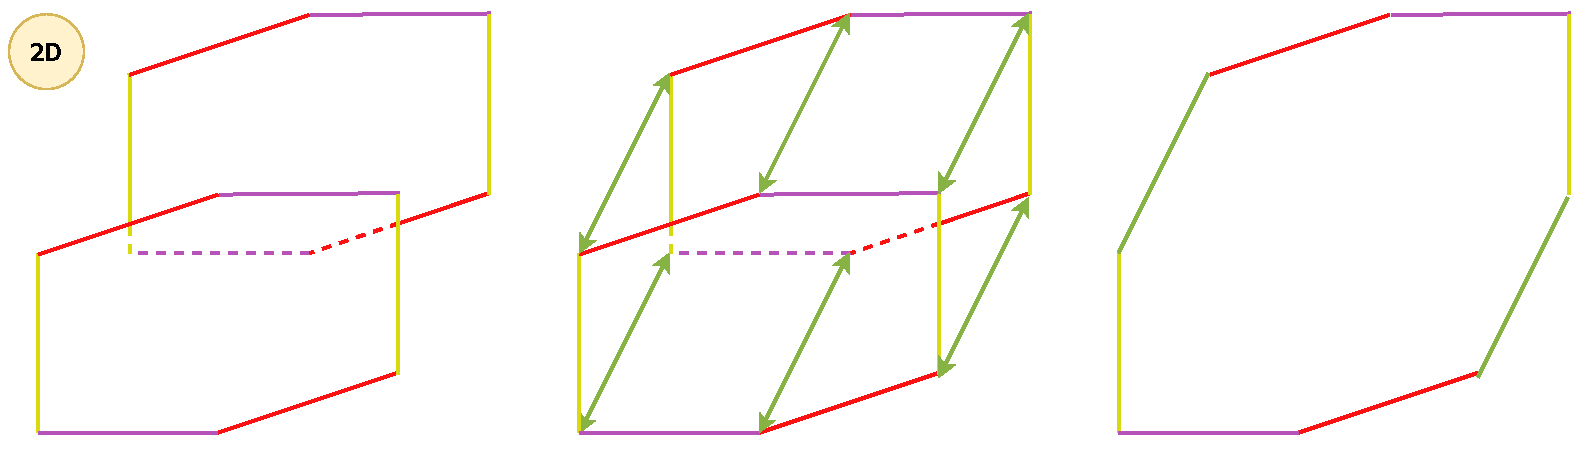
\includegraphics[trim={0 0 0 0},clip,width=1\linewidth]{img/chapter_2/zonotope_edges_elimination_end.pdf}

    \caption{After exactly $m-2$ iterations, the returned edges are exactly the zonotope edges.}
    \label{fig:zonotope_edges_elimination_end}
\end{figure}


\clearpage 
\subsubsection*{The EdgeEnum algorithm}
In the next algorithms, an edge of the $m$-cube can be represented by two $m$-dimensional vectors: a direction vector and an initial position point.
Algorithm \ref{alg:cube_edge_enumeration} computes how to create a new set of edges in one higher dimension $d+1$ from a set of given edges in $\IRd$, using the construction of edges of a higher dimensional cube. Algorithm \ref{alg:edge_enum}, called EdgeEnum, constructs zonotope edges following the reasonning previously described.
\begin{figure}[!ht]
    \centering
    \begin{minipage}{1.0\linewidth}
        \begin{algorithm}[H]
            \SetAlgoLined
            \KwData{$\textup{E}_d$ a set of edges in $\mathbb{R}^d$}
            \KwResult{$\textup{E}_{d+1}$ a set of edges in $\mathbb{R}^{d+1}$}
            
            \SetKwFunction{FMain}{duplicateAndLinkEdges}
            \SetKwProg{Fn}{Function}{:}{}
            \Fn{\FMain{$\textup{E}_d$}}{
                $\text{E}_{d+1} \gets \emptyset$\;
                \ForEach{$\mathbf{e}\in \textup{E}_d$}{
                    $\mathbf{e}_0 \gets \textup{embedInOneHigherDimension}(\mathbf{e})$\;
                    $\mathbf{e}_1 \gets \textup{translateAlongNewDimensionBy1}(\mathbf{e}_0)$\;
                    $v_0^1,\, v_0^2 \gets \textup{verticesAtExtremities}(\mathbf{e}_0)$\;
                    $v_1^1,\, v_1^2 \gets \textup{verticesAtExtremities}(\mathbf{e}_1)$\;
                    $\mathbf{e}_{01}^1 \gets \textup{createEdge}(v_0^1, v_1^1)$\;
                    $\mathbf{e}_{01}^2 \gets \textup{createEdge}(v_0^2, v_1^2)$\;
                    $\text{E}_{d+1} \gets \text{E}_{d+1} \cup \{\mathbf{e}_0, \mathbf{e}_1, \mathbf{e}_{01}^1, \mathbf{e}_{01}^2\}$;
                }        
                \Return{$\textup{E}_{d+1}$}
            }
            \textbf{End Function}
            \caption{Duplication, translation and link of edges}
            \label{alg:cube_edge_enumeration}
        \end{algorithm}
    \end{minipage}
\end{figure}
\begin{figure}[!ht]
    \centering
    \begin{minipage}{1.0\linewidth}
        \begin{algorithm}[H]
            \SetAlgoLined
            \KwData{A matrix $N \in \mathbb{R}^{n\times m}$, with $n\geq 2$ and $m\geq 2$}
            \KwResult{Edges of the zonotope $\Zono(\mathbf{c}, N)$}
            $d\gets 2$\;
            $N_d\gets N[:,:d]$\;            
            $\text{Edges}(\Cube_d)\gets \{\text{edges of the 2D cube}\}$ \tcp{$\Cube_d$ is the cube $[0,1]^d$.}
            $\text{Edges}(\Zono(\mathbf{c}, N_d))\gets \{\mathbf{c} + N_d\mathbf{e} \mid \mathbf{e}\in\text{Edges}(\Cube_d)\}$ \;
            
            $d\gets 3$\;
            \While{$d \leq m$}{
                $N_d\gets N[:,:d]$\;
                $\text{Edges}(\Cube_{d-1}) \gets \text{Edges}(\Cube_d)$\;
                $\textup{Edges}(\Cube_{d}) \gets \textup{duplicateAndLinkEdges}(\textup{Edges}(\Cube_{d-1}))$ \tcp{cf. algorithm \ref{alg:cube_edge_enumeration}}
                
                $\text{Edges}(\Zono(\mathbf{c}, N_d))\gets \{\mathbf{c} + N_d\mathbf{e} \mid \mathbf{e}\in\text{Edges}(\Cube_d)\}$ \;
        
                \ForEach{group of parallel edges $G\in\textup{Edges}(\Zono(\mathbf{c}, N_d))$}{
                    \ForEach{$\mathbf{c} + N_d\mathbf{e} \notin \textup{ext}(\textup{conv}(G))$}{
                        $\text{Edges}(\Cube_d) \gets \text{Edges}(\Cube_d) / \{\mathbf{e}\}$\;
                    }
                    
                }
                
                $d\gets d+1$
            }
            
            $\text{Edges}(\Zono(\mathbf{c}, N_d))\gets \{\mathbf{c} + N_d\mathbf{e} \mid \mathbf{e}\in\text{Edges}(\Cube_d)\}$ \;
            \Return{$\textup{Edges}(\Cube_d),\, \textup{Edges}(\Zono(\mathbf{c}, N_d))$}
            \caption{EdgeEnum: Zonotope edge enumeration algorithm}
            \label{alg:edge_enum}
        \end{algorithm}

    \end{minipage}
\end{figure}


% \begin{table}[]
%     \centering
%     \begin{tabular}{|l|l|l|l|l|}
%     \hline
%     $(n,\,m)$ & Naive & HSM  & Edges & Edges (parallelized) \\ \hline
%     (6,7)       & $0.019\pm0.001$  & $0.023\pm 0.002$ & $0.033\pm 0.002$ & $\mathbf{0.022\pm 0.010}$   \\ \hline
%     (6,9)       & $0.159\pm 0.011$ & $\mathbf{0.024\pm 0.273}$ & $0.216\pm 0.016$ & $0.083\pm 0.024$   \\ \hline
%     (7,8)       & $0.232\pm 0.025$ & $0.246\pm 0.022$ & $0.203\pm 0.014$ & $\mathbf{0.062\pm 0.008}$   \\ \hline
%     (7,9)       & $0.933\pm 0.064$ & $1.216\pm 0.005$ & $0.754\pm 0.026$ & $\mathbf{0.203\pm 0.019}$   \\ \hline
%     (8,8)       & $0.761\pm 0.091$ & $0.764\pm 0.078$ & $0.365\pm 0.019$ & $\mathbf{0.101\pm 0.012}$   \\ \hline
%     (8,9)       & $6.054\pm 0.577$ & $6.516\pm 0.885$ & $2.375\pm 0.101$ & $\mathbf{0.636\pm 0.042}$   \\ \hline
%     \end{tabular}
%     \caption{Mean and standard deviation of time computation in seconds for $20$ random zonotopes generated per $(n,\,m)$ combination
%     with $n$ is the dimension of the zonotope $Z$ and $m$ the dimension of $C^m$. A convertion to vertices is applied on the results of HSM and Edges and 
%     taken into account in the time computation. All the tests have been computed using a Dell XPS Windows 11 computer using a 16-core Intel i9 processor.}
% \end{table}


\section{Theoretical complexity}
\label{time_complexity_edgeenum}
In this section, various theoretical results about our new algorithm are shown, using complexity as the main tool of comparison. While a thorough time and space complexity analysis is given, the asymptotic time growth as the number of generators increases is our main interest since it is related to a larger number of muscles considered to compute the torque feasible set. This means that $n$, the dimension of the ambiant space the zonotope lives in is considered to be of fixed value while the number of generators $m$ is assumed to be large in general.

Before diving into the analysis, we recall some basics over algorithmic terms and the asymptotic growth usage:


\paragraph*{Asymptotic growth and Big $O$ notation.}
An \emph{asymptotic growth} describes how a function behaves as its input becomes very large and we denote by a \emph{Big $O$} notation the dominant terms. For instance, the function $f\colon \mathbb{N} \rightarrow \mathbb{N}$ defined by $f(n) = 4n^5 + n^5\log (n)$ is dominated by the term $n^5\log(n)$, meaning that when $n$ tends to $+\infty$, $f(n)$ will approximately have the same growth rate as the function $n\mapsto n^5\log(n)$. We use the Big $O$ notation to precise this growth rate comparison by stating $f$ is in $O(n^5\log(n))$ or $f(n) = O(n^5\log(n))$. To compare the asymptotic growth of two functions, their respective growth are calculated and the ratio of these rates is evaluated to decide which of the two has a slower growth than the other. If the ratio tends to a constant value, then both algorithms have asymptotically the same growth. More generally, we consider $O$ to represent a class of functions which are bounded by a given formula: in our example, $f$ is \emph{in} $O(n^5\log(n))$ but it is also in higher classes such as $O(n^6)$ or $O(n^{20})$.

\paragraph*{Algorithmic complexity.} For algorithms, two types of complexity are commonly described: the \emph{time} and the \emph{space} complexity. The time complexity evaluates theoretically the required time of each operation, while the space complexity evaluates the required storage. 

\paragraph*{Efficient algorithm.}
An algorithm is \emph{polynomial} or \emph{efficient} if its time complexity is upper bounded by a polynomial expression of both the input size and the output size (\cite{fukudaZonotopeConstructionMinkowski2004a}).  In other words, the running time of the algorithm doesn't grow exponentially as the input size increases, making it generally efficient for solving problems. For algorithms related to zonotope vertex enumeration, the input size corresponds to the number of dimensions times the number of generators (so essentially the number of elements in the generator matrix), while the output size include the number of vertices, faces, generator dimensions, etc.

\paragraph*{Compact algorithm.}
An algorithm is \emph{compact} if its space complexity in polynomial in the input size: this means that a compact algorithm does not store \emph{all} of the output and can stream the results directly without keeping in storage the output. It is a very useful property, especially when the size of the output is huge.
In the literature, two main approaches can be found: reverse-search-based algorithms and iterative algorithms. Algorithms are theoretically more valuable if they are compact, especially in high dimensions, so this approach is preferred and commonly found \cite{avisPivotingAlgorithmConvex}, \cite{guCounterfactualIdentificationLatent2022} and \cite{radaNewAlgorithmEnumeration2018}, but it should not exclude non-compact algorithms depending on the application context.

\paragraph*{Optimal algorithm.}
An algorithm is \emph{optimal} (in time and/or in space) if its complexity has been proven to be the lowest ever reachable. 
For instance, it has been recalled in theorem 3.2 of Ferrez et al. \cite{ferrezSolvingFixedRank2005a} that there exists a time-optimal algorithm which enumerate all zonotope vertices in time $O(m^{n-1})$, which has been implemented in 1983 by Edelsbrunner et al. \cite{edelsbrunnerConstructingArrangementsLines1983}.
Unfortunately, such an optimal algorithm may not be practical \cite{ferrezSolvingFixedRank2005a}: firstly, it uses an incremental strategy which requires to store all extreme points of a subproblem based on a lesser number of generators. Secondly, it is complicated to implement and needs to store all faces and their incidence (\emph{i.e.} if the intersection if two faces is another face or not). In other words, Edelsbrunner et al.'s algorithm is time optimal and efficient, but space defficient.


In our context, we mainly care about time efficiency. As the next theorems show, our new algorithm is time efficient even when considering the edges-to-vertices transition. It is also space efficient but it is not compact. 
Before diving into complexity calculations, let's describe a very useful result concerning the number of specific faces in a zonotope. A zonotope $\Zono$ in dimension $n$ has $n-1$ type of faces: the $0$-faces are called \emph{vertices}, the $1$-faces \emph{edges}, the $(n-2)$-faces \emph{ridges}, and the $(n-1)$-faces \emph{facets}. In specific cases such as in dimension $2$, the edges correspond to the facets. In 3D, edges correspond to ridges.

\begin{lemmabox}{Upper bound on the number of $k$-faces of a zonotope}{nb_k_faces_zonotope}
    For $G\in\IRnm$, the number of $k$-faces of the zonotope $\Zono(G)$ for $k=1,\dots, n-1$ is upper bounded by $f_k(\Zono)$ such that
    $$f_k(\Zono) = 2\binom{m}{k} \sum_{i = 0}^{n-k-1} \binom{m-k-1}{i}$$
    The bound is atteigned if $\Zono$ is in general position.
\end{lemmabox}
\begin{proof}
    This result can be found with proof in \cite{fukudaZonotopeConstructionMinkowski2004a}, \cite{donohoCountingFacesRandomlyProjected2010} and \cite{grunbaumConvexPolytopes2013}.
\end{proof}

\subsection{Time complexity}
\begin{theorembox}{Time complexity of EdgeEnum}{time_complexity}
    For a $n$-zonotope $\Zono$ with $m$ generators in general position, the edge enumeration algorithm is in time complexity
    $$O\left( nm^2f_1(\Zono)\right)$$
    where $f_1(\Zono)$ denotes the number of edges of $\Zono$.
    % $$O\left( nm^2f_1(\Zono) +  f_1(\Zono)\log\left(\frac{f_1(\Zono)^m}{m!}\right)\right)$$
\end{theorembox}
\begin{proof}
    Each iteration of the algorithm (\emph{i.e.} $d=3,\dots, m$) consider a new zonotope $\Zono_d$ generated by the first $d$ columns of the generator matrix $G\in\IRnm$ and construct its edges based on the set of edges of $\Zono_{d-1}$. We are going to thoroughly analyze the time computation of every step in the algorithm:

    \textbf{1. Embed, duplicate and translate edges:} In the first inner-loop, a new dimension is added to the edges of $\Zono_{d-1}$, which can be done by concatenating a $0$ to both the direction and position vector describing each of them. These embedded edges are then duplicated and the copied versions have their direction and position last coordinates mutated to $1$. New edges are created by linking the respective extremity points from the embedded edges to their translate. This whole step can be done in time complexity $O(1)$ for each substep, in a loop over each of the previous edges, so it is $O(f_1({\Zono_{d-1}}))$.

    \textbf{2. Grouping edges by parallelism:} The newly created set of edges consists of exactly $4f_1(\Zono_{d-1})$ edges. Since colinearity between cube edges is preserved under linear transformation, grouping edges of zonotope $\Zono_d$ by parallelism only requires to group the cube edges by directions. In Python, using a dictionnary structure, the grouping process is $O(f_1(\Zono_{d-1}))$.
    
    \textbf{3. Applying the convex hull over each group of edges:} Each group of edge consists of $2f_1(\Zono_{d-1}) / (d-1)$ edges, and there are $d$ groups. For each group, each edge will be projected onto $\IRn$ via the generator matrix of $\Zono_d$. This corresponds to one matrix-vector operation of time complexity $O(nd)$ per edge. The projection done, the orthogonal projection of the origin in $\IRn$ onto the line spanned by the projected edge is computed in time complexity $O(n)$ (the dimension of the ambiant space where the line is defined). The convex hull of the projected edges is computed as the convex hull of the orthogonal projections of the origin onto the lines spanned by the edges. Let's consider the time complexity of Chan's convex hull algorithm in $n$ dimensions. It is an output-sensitive algorithm, which means that its complexity depends on the size of the output. Its time complexity is $O(n_v\log h)$ with $n_v$ the number of given points and $h$ the known number of points on the convex hull. Since the zonotope $\Zono_d$ is in general position,  the number of edges in each group is $f_1(\Zono_d) / d$. The total time complexity of step $3$ is then of order
    $d (\frac{2f_1(\Zono_{d-1})}{d-1}nd + \frac{2f_1(\Zono_{d-1})}{d-1}n + \frac{2f_1(\Zono_{d-1})}{d-1}\log(\frac{f_1(\Zono_{d})}{d}))$, which is
    $O(f_1(\Zono_{d-1}) nd +f_1(\Zono_{d-1})  \log(f_1(\Zono_{d}) / d))$.

    After $d$ iterations, the complexity is of order $\sum_{d=3}^m f_1(\Zono_{d-1}) nd +  f_1(\Zono_{d-1}) \log(f_1(\Zono_d) / d)$ and since $d \leq m$ and $f_1(\Zono_d) \leq f_1(\Zono)$, we have the following upper bound:
    \begin{align*}
        \sum_{d=3}^m f_1(\Zono_{d-1}) nd +  f_1(\Zono_{d-1}) \log(f_1(\Zono_d) / d) &\leq  f_1(\Zono) \left[ n \sum_{d=3}^m d + \sum_{d=3}^m \log\left(\frac{f_1(\Zono)}{d}\right) \right] \\
        &\leq  f_1(\Zono) \left[ nm\frac{m+1}{2} +  \log\left(\prod_{d=1}^m\frac{f_1(\Zono)}{d}\right) \right] \\
        &\leq  f_1(\Zono) \left[ n\frac{m^2+m}{2} +  \log\left(\frac{f_1(\Zono)^m}{m!}\right) \right]
    \end{align*}
    So the edge-based algorithm is upper bounded in $O\left( nm^2f_1(\Zono) +  f_1(\Zono)\log\left(\frac{f_1(\Zono)^m}{m!}\right)\right)$.

    The second part of the proof is to show that $nm^2f_1(\Zono)$ is the dominant term in this upper bound. Let's show that for any growth of $n$ and $m$, $f_1(\Zono)\log\left(\frac{f_1(\Zono)^m}{m!}\right) / (nm^2f_1(\Zono))$ is upper-bounded by a function whose growth tends to be constant (meaning it is $O(1)$).
    \begin{align*}
        \frac{f_1(\Zono)\log\left(\frac{f_1(\Zono)^m}{m!}\right)}{nm^2f_1(\Zono)} 
        &\leq \frac{1}{nm^2}\log\left(f_1(\Zono)^m\right) \\
        &= \frac{1}{nm}\log\left(f_1(\Zono)\right) \\
        &= \frac{1}{nm} \log\left(2\binom{m}{1}\sum_{i=0}^{n-2}\binom{m-2}{i}\right),\quad \text{using theorem \ref{th:nb_k_faces_zonotope}} \\
        &\leq \frac{1}{nm} \log\left(m2^{m-1}\right),\quad \text{using } \sum_{i=0}^{n-2}\binom{m-2}{i} \leq \sum_{i=0}^{m-2}\binom{m-2}{i} = 2^{m-2}  \\
        &= \frac{ \log(m)}{nm} + \frac{ (m-1)\log(2)}{nm} \\
    \end{align*}
    There are now three cases to study:
    \begin{enumerate}[noitemsep]
        \item {$n \rightarrow +\infty$ and $m$ grows at a smaller rate than $n$ ($\lim_{m,n\to +\infty}\frac{m}{n} = 0$): 
        $$\lim_{m,n\to +\infty}\frac{ \log(m)}{nm} = \lim_{m,n\to +\infty}\frac{1}{nm}  = 0\quad \text{and} \quad \lim_{m,n\to +\infty} \frac{ (m-1)\log(2)}{nm} = \lim_{n\to +\infty}\frac{1}{n}  =  0$$
        }
        \item  {$m \rightarrow +\infty$ and $n$ grows at a smaller rate than $m$ ($\lim_{m,n\to +\infty}\frac{n}{m} = 0$): 
        $$\lim_{m,n\to +\infty}\frac{ \log(m)}{nm} = \lim_{m,n\to +\infty}\frac{1}{nm}  = 0\quad \text{and} \quad \lim_{m,n\to +\infty} \frac{ (m-1)\log(2)}{nm} = \lim_{m,n\to +\infty}\frac{1}{n}  =  0$$
         }
         \item  {$m \rightarrow +\infty$ and $n \rightarrow +\infty$ at an equivalent rate ($\lim_{m,n\to +\infty}\frac{n}{m} = C$, for $C$ a positive constant): 
         $$\lim_{m,n\to +\infty}\frac{ \log(m)}{nm} = \lim_{m,n\to +\infty}\frac{1}{nm}  = 0\quad \text{and} \quad \lim_{m,n\to +\infty} \frac{ (m-1)\log(2)}{nm} = \lim_{m,n\to +\infty}\frac{1}{n}  =  0$$
          }
    \end{enumerate}
    All cases confirm that $f_1(\Zono)\log\left(\frac{f_1(\Zono)^m}{m!}\right)$ is dominated in growth by $nm^2f_1(\Zono)$ for any cases of growth for $m$ and $n$. This means that the complexity of our edge enumeration algorithm is $O(nm^2f_1(\Zono))$.
\end{proof}

Now, let's show an intermediate result which will be used in the proof of the next theorem \ref{th:time_complexity_n_fixed}.
\begin{lemmabox}{Upper asymptotic growth for the number of $k$-faces}{big_O_nb_k_faces} For $Z$ a $n$-zonotope with $m$ generators in general position, then $f_k(\Zono)$ the number of $k$-faces of $\Zono$ when $k$ and $n$ are fixed and $m$ is large has an asymptotic growth upper-bounded in $O(m^{n-1})$.
\end{lemmabox}
While it was already well-known that the number of vertices $f_0(\Zono)$ is asymptotically bounded in $O(m^{n-1})$ (proven by Zaslavsky in \cite{zaslavskyFacingArrangementsFaceCount1975}), our result extends this finding to higher dimensions  in order to find an asymptotic upper-bound for the number of $k$-faces, as long as $k$ and $n$ are considered constant. This theorem stipulates that the number of vertices, edges, ridges, hyperplanes and all type of $k$-faces of a general zonotope are all upper bounded by the same type of growth as $m$ increases. We will use this theorem later to compute the asymptotic growth of our edge enumeration algorithm in the case of $n$ fixed, which will help us to compare our algorithm against the state-of-the-art.
\begin{proof}We shall proceed by finding an upper bound of $f_k(\Zono)$ which is $O(m^{n-1})$ for $n$ fixed. First, notice that for $0\leq n\leq m$, $m^n$ is an upper bound of $\binom{m}{n}$:
    \begin{align}
        \label{ineq:upper_bound_binomial}
        \binom{m}{n} &= \frac{m!}{n!(m-n)!} = \frac{1}{n!} \cdot m(m-1)(m-2)\dots (m-n+1)  \leq m^n
    \end{align}
    
    Also, when considering $m$ large and $k, n$ fixed, it is reasonable to assume 
    $(n-k-1) \leq (m-k-1)/2$ so that 
    \begin{align}
        \label{ineq:upper_bound_binomial_half}
        \binom{m-k-1}{i}\leq \binom{m-k-1}{n-k-1},\quad \text{for any $i = 1, \dots, n-k-1$}
    \end{align}
    
    Hence the following:
    \begin{align*}
        f_k(\Zono) &= 2\binom{m}{k}\sum_{i=0}^{n-k-1}  \binom{m-k-1}{i} \\
        &\leq 2\binom{m}{k}\ \sum_{i=0}^{n-k-1} \binom{m-k-1}{n-k-1},\quad  \text{using inequality \ref{ineq:upper_bound_binomial_half}} \\
        &\leq 2m^k (m-k-1)^{n-k-1} (n-k),\quad \text{using inequality \ref{ineq:upper_bound_binomial}}
    \end{align*}
    The last inequality is equivalent to state that $f_k(\Zono)$ is $O(m^{n-1})$, for $k, n$ fixed and $m$ large.
\end{proof}

\begin{theorembox}{Time complexity of EdgeEnum when $n$ is fixed}{time_complexity_n_fixed}
    If $n$ is fixed and $m$ is large, the time complexity of the edge enumeration is $O\left( m^{n+1} \right)$. Also, this means that EdgeEnum is an algorithm of polynomial time when $n$ fixed.
\end{theorembox}
\begin{proof}
    This directly is deduced from theorem \ref{th:big_O_nb_k_faces} stating that the number of faces $f_1(\Zono)$ is $O(m^{n-1})$ when $n$ is fixed. Using the time complexity of EdgeEnum in theorem \ref{th:time_complexity}, we have for $n$ fixed:
    $O(nm^2f_1(\Zono)) = O(m^2m^{n-1}) = O(m^{n+1})$.
\end{proof}

\subsubsection*{From edges to vertices}
\begin{theorembox}{Time complexity to convert edges to vertices}{time_complexity_edge_to_vertex}
    For a $n$-zonotope $\Zono$ with $m$ generators in general position, the time complexity of an algorithm enumerating vertices from its edges is in $O(nmf_1(\Zono))$.
\end{theorembox}
\begin{proof}
Every edge of $\Zono$ is linked to two vertices, which corresponds to its extremities. The transformation of all the edges to vertices can be realized in time complexity $O(f_1(\Zono)nm)$: indeed, the two extremities of each cube edge must be projected via the generator matrix so this accounts for $2f_1(\Zono)nm$ $O(1)$ steps. An iteration of all these vertices can be done as well to ensure the uniqueness of each vertex (2 edges can lead to a common vertex!). This step of verification can be done in $O(f_1(\Zono))$ in Python, using a hash structure.
\end{proof}
Since $nm^2f_1(\Zono)$ dominates $nmf_1(\Zono)$, we can safely say that the convertion step from edges to vertices does not have a theoretical time impact in a worst-case scenario if this step is added after the edge-enumeration algorithm.

\subsection{Space complexity}
\begin{theorembox}{Space complexity of EdgeEnum}{space_complexity}
    For a $n$-zonotope $\Zono$ with $m$ generators in general position, the edge enumeration algorithm is in space complexity
    $$O\left( n^2m^2f_1(\Zono)\right)$$
    where $f_1(\Zono)$ denotes the number of edges of $\Zono$.
    % $$O\left( nm^2f_1(\Zono) +  f_1(\Zono)\log\left(\frac{f_1(\Zono)^m}{m!}\right)\right)$$
\end{theorembox}
\begin{proof}
    The algorithm starts with a matrix in $\IRnm$ so requires an input space in $O(nm)$. In the first steps; the definition of the $2$-cube edges and their projection is in $O(n)$ clearly.

    \textbf{1. Embed, duplicate, translate edges:} 
    A cube edge can be described in two parts: a direction and a position in $\IRm$. A direction of a cube edge is in $O(1)$, since it is necessarily assimilated to a vector $e = (0, \dots, 0, 1, 0,\dots, 0) \in \IRm$ (due to parallelism of edges to the canonical basis of $\IRm$). The position, however, can be more general so let's take a worst case scenario of $O(m)$.

    Each edges at the begining of the loop is copied, then embedded, duplicated and new edges are created. There are maximum $f_1(\Zono_{d-1})$ edges at the begining so these steps require a space in $O((d-1)\cdot f_1(\Zono_{d-1}) + 3\cdot d\cdot f_1(\Zono_{d-1})) = O(d\cdot f_1(\Zono_{d-1}))$.

    \textbf{2. Grouping edges by parallelism:} 
    First, all newly created edges need to be projected onto the space generated by $N_d$, so it gives a new set of projected edges in $O(ndf_1(\Zono_{d-1}))$. Using a dictionnary in Python to pair edges with a projected direction (in this case corresponding to a generator of $N_d$), this requires $O(d)$ space with $d$ corresponding to the number of generators in the current iteration. The total space in this step is thus in $O(ndf_1(\Zono_{d-1}))$.
    
    \textbf{3. Applying the convex hull over each group of edges:} For each of the $d$ group of edges (consisting of $O(nf_1(\Zono_{d-1}))$ edges), Chan's convex hull algorithm has a space time complexity of $O(n\cdot nf_1(\Zono_{d-1})) = O(n^2 f_1(\Zono_{d-1}))$. This leads to a total space complexity of $O(dn^2f_1(\Zono_{d-1}))$.

    To conclude, since $d\leq m$ and $f_1(\Zono_d) \leq f_1(\Zono_m)$, we have for all the loops a space complexity in $O(nm + n + \sum_{d=3}^m df_1(\Zono_{d-1}) + ndf_1(\Zono_{d-1}) + dn^2f_1(\Zono_{d-1}))$ and since the terms in the sum are dominated by $dn^2f_1(\Zono_{d-1})$, itself dominated by $mn^2f_1(\Zono_d)$, we have a total space complexity of $O(n^2 m^2 f_1(\Zono_d))$.
\end{proof}

This leads directly to the following result:
\begin{theorembox}{Space complexity to convert edges to vertices}{space_complexity_edge_to_vertex}
    For a $n$-zonotope $\Zono$ with $m$ generators in general position, the space complexity of an algorithm enumerating vertices from its edges is in $O(nf_1(\Zono))$.
\end{theorembox}
\begin{proof}
    Consider $f_1(\Zono)$ the maximum number of edges of a zonotope $\Zono$. The input of the convertion algorithm is thus $O(nf_1(\Zono))$ which is represented as a dictionnary of a zonotope generator and a position vector in $\IRn$. Now, for each of these edges we shall create extremal vertices, which include the position vector and the addition of the position vector and the associated generator, so that the space complexity is still in $O(nf_1(\Zono))$.
\end{proof}
This ensures that the total space complexity from the edge enumeration to the vertex enumeration is $O(n^2m^2f_1(\Zono))$.

\begin{theorembox}{Space complexity of EdgeEnum when $n$ is fixed}{space_complexity_n_fixed}
    If $n$ is fixed and $m$ is large, the space complexity of the edge enumeration is $O\left( m^{n+1} \right)$. Also, this means that EdgeEnum is an algorithm of polynomial space when $n$ fixed.
\end{theorembox}
\begin{proof}
    Since the space complexity is $O(n^2m^2f_1(\Zono))$ and that $f_1(\Zono)$ is $O(m^{n-1})$ when $n$ fixed, we have that $O(n^2m^2f_1(\Zono))$ is $O(m^{n+1})$, which is a polynomial bounding both the input size $nm$ and the output size $O(m^{n-1})$.
\end{proof}

% When $n$ is fixed, the time 
% Contrary to the time complexity, here the space complexity is not polynomially bounded. Indeed, consider the number of edges of 

\subsection{Time-theoretic comparison with other algorithms}
The proposed algorithm exhibits time complexity of $O(m^{n+1})$, while the optimal lower bound is $O(m^{n-1})$. Despite this discrepancy, the algorithm demonstrates several desirable properties, such as being easily implementable with standard scientific programming languages and packages. Nevertheless, there exist another significant algorithms focused on this problem that we shall described succintly.

\paragraph*{Avis and Fukuda's pivoting algorithm \cite{avisPivotingAlgorithmConvex}.}
The \emph{pivoting} algorithm, a type of \emph{reverse-search} algorithms created by the same authors, was initially created to enumerate the vertices of a polytope described by a set of inequalities. Broadly, the algorithm starts with a vertex, then a neighboring vertex is found through a \emph{pivot rule}, which decides which vertex to visit next based on the current vertex and the polytope structure. The new vertex is then marked as visited, and through iteration over each newly found vertex, all polytope vertices are enumerated. Numerous variant of this algorithm are possible by adapting the pivot rule. This algorithm also has been extended to compute vertices of a zonotope using only its generators, and has also been implemented in C++ with a Python wrapper in \emph{libzonotope} by Ingvason \cite{yngvassonLibzonotope}. Also, an effective parallelized variant of the pivoting algorithm as been done by Weibel in 2010 \cite{weibelImplementationParallelizationReverseSearch2010}, and can be used through the C++ implementation \emph{Minksum} \cite{weibelMinksum}.

The initial reverse-search algorithms were not described as a zonotope vertex enumeration. 
They were implemented to solve two kinds of problems: computing the convex hull of a set of points and computing the \emph{cell enumeration of a central hyperplane arrangement problem}. 
The latest corresponds to an alternative description of a zonotope. There is a one-to-one correspondance between the combinatorial face structure of a zonotope and its central hyperplane arrangement. The idea is to consider the hyperplanes normal to each generator of a zonotope: the \emph{cells} of this arrangement correspond to the regions created by the hyperplanes intersections. Describing and enumerating these cells (via a sign vector as shown in \cite{ferrezSolvingFixedRank2005a}, \cite{radaNewAlgorithmEnumeration2018}) is equivalent to finding the vertices of a zonotope. Figures \ref{fig:zonotope_hyperplane_arrangement} and \ref{fig:zonotope_hyperplane_arrangement2} summarize this correspondance by giving some intuition on how to construct it from a zonotope and how to compute vertices from the regions of such an arrangement. This construction generalizes well for zonotope generators in any dimension. 
For a more profound understanding of this duality and further details on this correspondance, the reader is invited to read the \emph{Duality} section of Ferrez et al. \cite{ferrezSolvingFixedRank2005a}, or more generally in Grünbaum's dedicated chapter \emph{Arrangement of hyperplanes} \cite{grunbaumConvexPolytopes2013}.

\begin{figure}[!htb]
    \captionsetup{justification=centering}
    \begin{minipage}{0.49\linewidth}
        \centering
        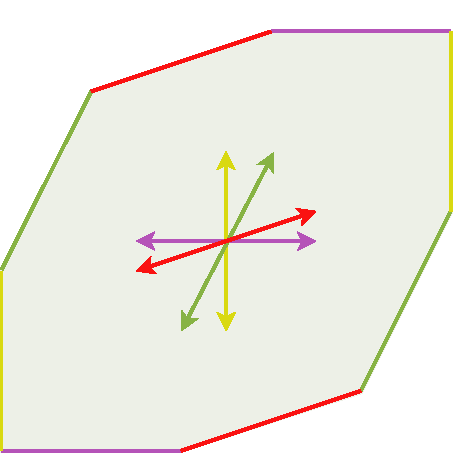
\includegraphics[trim={0 0 0 10},clip, width=0.6\linewidth]{img/chapter_2/zonotope_edges_parallel_generator.pdf}
    \end{minipage}
    \hfill
    \begin{minipage}{0.49\linewidth}
        \centering
        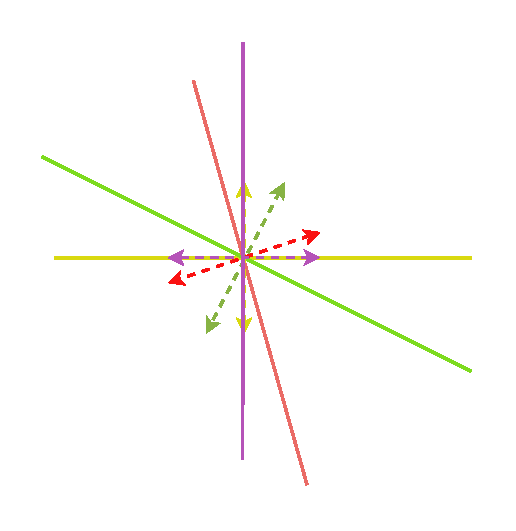
\includegraphics[trim={10 50 10 50},clip,width=0.8\linewidth]{img/chapter_2/central_arrangement.pdf}
    \end{minipage}
    \caption{To the left: a zonotope with four generators. To the right: the normal hyperplanes to each generator. This corresponds to its \emph{central hyperplane arrangement}.}
    \label{fig:zonotope_hyperplane_arrangement}
\end{figure}
\begin{figure}[!htb]
    \captionsetup{justification=centering}
    \centering
    
    \begin{minipage}{0.49\linewidth}
        % \centering
        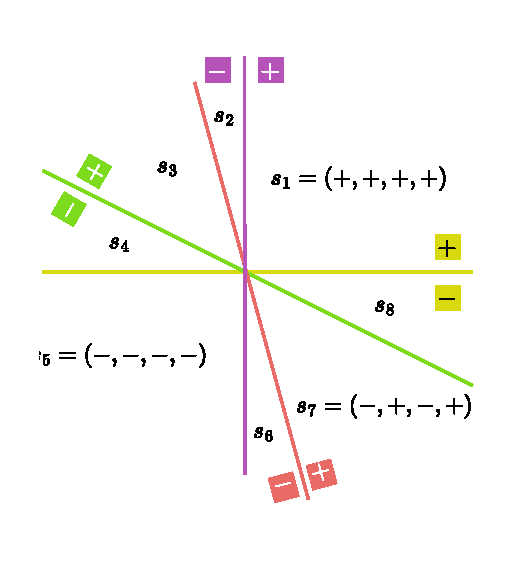
\includegraphics[trim={0 20 0 20},clip, width=0.9\linewidth]{img/chapter_2/sign_vectors_zonotope.pdf}
    \end{minipage}
    \hfill
    \begin{minipage}{0.49\linewidth}
        % \centering
        \hfill
        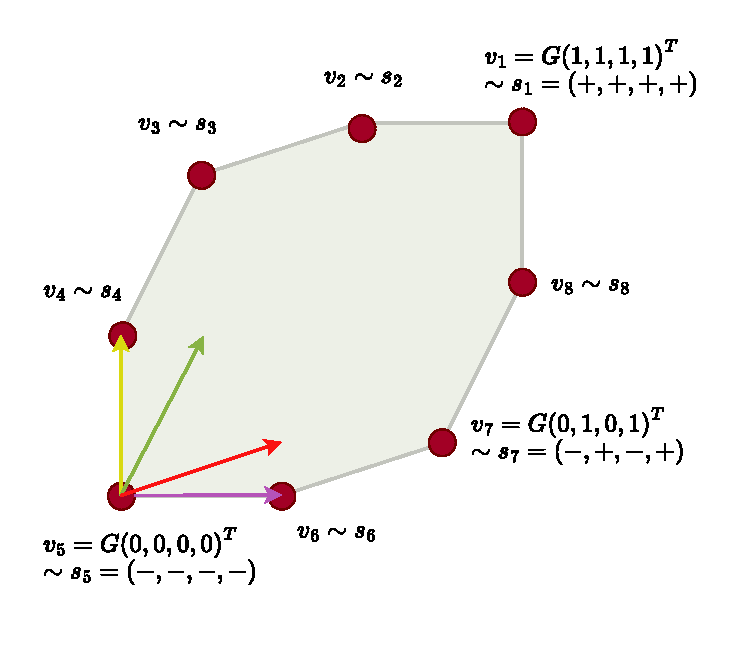
\includegraphics[trim={0 20 0 20},clip,width=1\linewidth]{img/chapter_2/zonotope_vertices_sign_vectors.pdf}
    \end{minipage}
    % 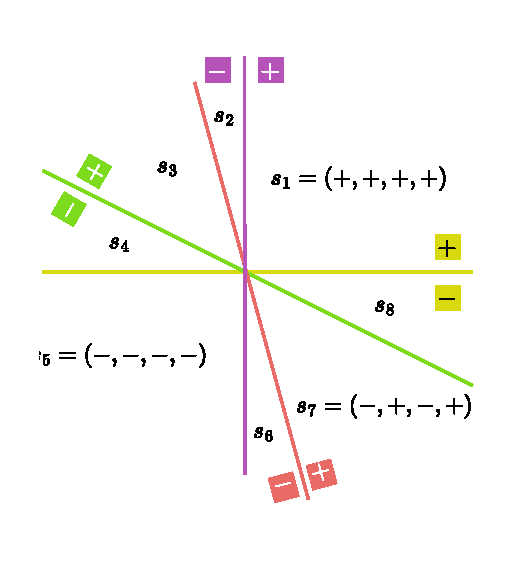
\includegraphics[trim={0 0 0 0},clip, width=0.5\linewidth]{img/chapter_2/sign_vectors_zonotope.pdf}
    \caption{Let $G$ be the matrix for the yellow, purple, red then green generators. In its central hyperplane arrangement, each region (or \emph{cell}) is represented by a sign vector $s_i$. Indeed, any $n$-dimensional space can be separated in exactly $2$ by any hyperplane. There are exactly as many cells as there are vertices in the underlying zonotope. Even more: they are in one-to-one correspondance, as shown by the symbol $\sim$.}
    \label{fig:zonotope_hyperplane_arrangement2}
\end{figure}

Thus, due to the simplicity of working with sign vectors, there is a focus in computation geometry to create algorithms dedicated to enumerate cells of a central hyperplane arrangements. The most recent ones include Rada and Cerny \cite{radaNewAlgorithmEnumeration2018}, Gu et Koenker \cite{guNonparametricMaximumLikelihood2020} but also Gu et al.'s 2022 algorithm \cite{guCounterfactualIdentificationLatent2022} whose practical time performance outperfoem the two previous one. We shall describe it next.

\paragraph*{Gu et al.'s GRS algorithm \cite{guCounterfactualIdentificationLatent2022}.}
This algorithm find cells of a central hyperplane arrangement iteratively over sub-dimensional arrangements. The main idea is to consider a \emph{witness} points in each cell, whose sign correspond the a cell description, then remove one hyperplane from the arrangement and project all other hyperplanes onto the space it generates. The previous witness points are then also projected onto it and they correspond to witness point of this sub-arrangement, up to duplication.
The figure \ref{fig:gu_et_al_algo} summarizes the process in two dimensions, where instead of projecting onto subspaces, the witness points are constructed iteratively.

\begin{figure}[!htb]
    \captionsetup{justification=centering}
    \centering
    
    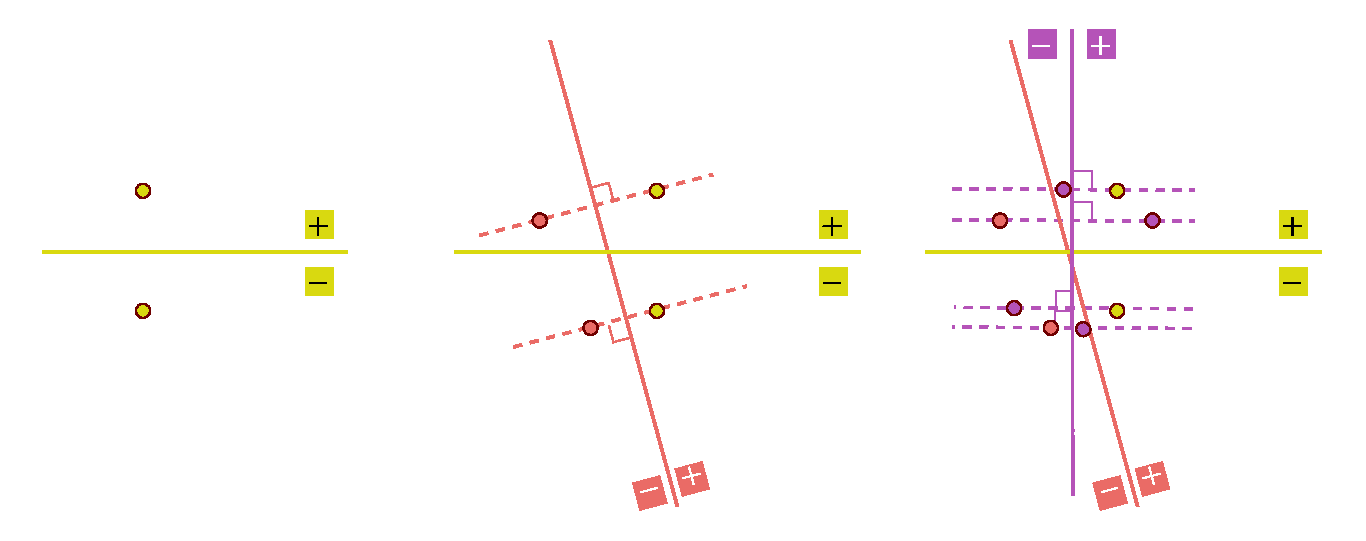
\includegraphics[trim={20 0 20 0},clip,width=1\linewidth]{img/chapter_2/gu_et_al_alg.pdf}
    % 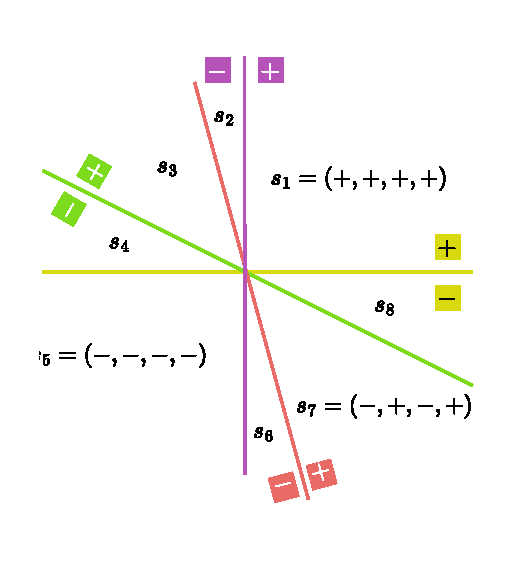
\includegraphics[trim={0 0 0 0},clip, width=0.5\linewidth]{img/chapter_2/sign_vectors_zonotope.pdf}
    \caption{On the left: two points are created, on the respective sides of the hyperplane. At the middle: another hyperplane is added and the previously created points are copied on the other side of the novel hyperplane. Gu et al found a distance computation to ensure that the new points are in the closest region. To the right: repeat with another added hyperplane and remove duplicates \emph{i.e.} with the same sign vector.}
    \label{fig:gu_et_al_algo}
\end{figure}

The two previous cell enumeration methods are interesting, in regard to the correspondance, but other algorithms exist to convert zonotope generators to a different representation, such as its bounding hyperplanes. However, since we concentrate on enumerating vertices, the conversion between bounding hyperplanes and vertices should be taken into account. Avis and Fukuda offer such a conversion algorithm in \cite{avisPivotingAlgorithmConvex} in time complexity $O(n_h n n_v)$, where $n$ is the dimension of $n_h$ hyperplanes, and $n_v$ is the number of vertices created by intersecting them. Such a method using bounding hyperplanes is the following:

\paragraph*{Gouttefarde and Krut's hyperplane shifting method (HS) \cite{gouttefardeCharacterizationParallelManipulator2010a}.}
The number of bounding hyperplanes of a zonotope $\Zono(n,m)$ in general position is $f_{n-1}(\Zono) = 2\binom{m}{n-1}$, \emph{i.e.} the $(n-1)$-dimensional faces of the $m$-cube projects directly onto the zonotope bounding hyperplanes. Since the position of each $(n-1)$-faces in the $m$-cube is known, there remain to project the position and the $(n-1)$-space via the generator matrix, then compute the normal vectors. Using symmetrty, the algorithm only requires to enumerate $\binom{m}{n-1}$ hyperplanes. Its time complexity is thus $O(\binom{m}{n-1})$, since all linear operations in the algorithm (computing normals, projecting etc.) are necessarily bounded by $\binom{m}{n-1}$. We shall use the Python implementation available in Skuric et al's package Pycapacity \cite{skuricPycapacityRealtimeTaskspace2023}.

We now present in table \ref{tab:theoretic_comparison_complexity} the time complexity the three presented methods against EdgeEnum. 

\begin{table}[!ht]
    \centering
    \begin{tabular}{|c||c|c|c|c|}
    \hline
    Algorithm & \makecell{Pivot \cite{avisPivotingAlgorithmConvex}} & \makecell{HS \cite{gouttefardeCharacterizationParallelManipulator2010a}} & \makecell{GRS \cite{guCounterfactualIdentificationLatent2022}} & \makecell{EdgeEnum} \\
    \hline
    \hline
    \makecell{Initial enumeration type} & Cell & Hyperplane & Cell & Edge \\ \hline
    \makecell{Time complexity} & $mf_0 \text{lp}(m,n$) & $\binom{m}{n-1}$ & $mf_0\text{mat}(m)$ & $nm^2f_1$ \\ \hline
    \makecell{Additional complexity \\ to convert to vertices} & $nmf_0$ & \makecell{$\binom{m}{n-1}nf_0$ \\ \small{described in \cite{avisPivotingAlgorithmConvex}}} & $nmf_0$ & $nmf_1$ \\ \hline
    \makecell{Total complexity \\ for $n$ fixed} & $m^{n+2.38}$ & $m^{2n-1}$ & $m^{n+1}$ & $m^{n+1}$ \\ \hline
    
    \end{tabular}
    \caption{Comparison of time complexity between combinatorially equivalent enumeration algorithms when considering a $n$-dimensional zonotope with $m$ generators in general position. $f_0$ corresponds to its maximal number of vertices and $f_1$ of its edges. Pivot denotes Avis and Fukuda's pivoting algorithm (\cite{avisPivotingAlgorithmConvex}), HS stands Gouttefarde and Krut's hyperplane shifting method (\cite{gouttefardeCharacterizationParallelManipulator2010a}) and GRS is Gu et al's (\cite{guCounterfactualIdentificationLatent2022}). $\text{lp}(m,n)$ stands for the time complexity to resolve a linear program of $m$ equations of $n$ variables, and $\text{mat}(m)$ denotes the time cost to determine whether two vectors of length m are identical. (\cite{cohenSolvingLinearPrograms2020}) created an algorithm solving a linear program of $m$ equations and $n$ variables in a time complexity of the matrix multiplication, so about $m^{2.38}$. Also, using a programming language such as R or Python, we have $\text{mat}(m) = m$. An algorithm for converting a set of $n_h$ hyperplanes to $f_0$ vertices has been created in time $O(n_h n f_0)$ in (\cite{avisPivotingAlgorithmConvex}). The total complexity of HS is computed using Stirling's approximation of $\binom{m}{n}$ when $m$ gets large as $\binom{m}{n-1} \approx m^{n-1}/(n-1)! = O(m^{n-1})$ if $n$ is fixed.}
    \label{tab:theoretic_comparison_complexity}
\end{table}

% \begin{table}[!ht]
%     \begin{tabular}{r|c|c|c}
%     Algorithm & Enumeration & Time complexity & as $n$ is fixed \\ 
%     \hline
%     \hline
%     Naive algorithm & Vertex & $2^m\log f_0(\Zono)$ & $2^mm$ \\ \hline

%     Avis and Fukuda, 1993 \cite{avisPivotingAlgorithmConvex} & Cell &  $mf_0(\Zono)\text{lp}(m, n) $  &  $m^{n+2.38}$ \\ \hline
    
%     Gouttefarde et al., 2010 \cite{gouttefardeCharacterizationParallelManipulator2010a} & Hyperplane &  ${m \choose n-1}^2 n f_0(\Zono)$ & $m^{3n-2}$ \\ \hline

%     Rada and Cerny, 2018 \cite{radaNewAlgorithmEnumeration2018} & Cell & $mf_0(\Zono)\text{lp}(m, n)$ & $m^{n+2.38}$ \\ \hline

%     Gu et Koenker, 2020 \cite{guNonparametricMaximumLikelihood2020} & Cell & \makecell{$f_0(\Zono)\text{lp}(m, n)$ \\ $+ mf_0(\Zono)\text{mat}(m)$}  & $m^{n+1.38}$ \\ \hline

%     Gu et al., 2022 \cite{guCounterfactualIdentificationLatent2022} & Cell & $mf_0(\Zono)\text{mat}(m)$ & $m^{n+1}$ \\ \hline

%     EdgeEnum, 2024 & Edge & $nm^2f_1(\Zono)$ & $m^{n+1}$ \\                     
%     \end{tabular}
%     \caption{Comparison of time complexity between combinatorially equivalent enumeration algorithms. $\text{lp}(m,n)$ denotes the time complexity to resolve a linear program of $m$ equations of $n$ variables, and $\text{mat}(m)$ denotes the time cost to determine whether two vectors of length m are identical.}
% \end{table}

% It should be noted that in 2018, Cohen et al. \cite{cohenSolvingLinearPrograms2020} created an algorithm solving a linear program of $m$ equations and $n$ variables in a time complexity of the matrix multiplication, so about $m^{2.38}$. Also, using a programming language such as R or Python, we have $\text{mat}(m) = m$.

% Applying these in the time complexities of the algorithms shows us that for $n$ fixed and $m$ large, Gu et al. 2022's algorithm and EdgeEnum have the same time complexities of order $O(m^{n+1})$. All other algorithms have bounds which are worse than Gu et al. and EdgeEnum.

It should be noted that the case of $m$ fixed and $n$ large is not of interest: if the number of generators $m$ is smaller than the dimension of the associated zonotope, then the enumeration of the zonotope vertices necessarily requires to enumerate \textbf{all} of the $m$-cube vertices (which amounts to $2^m$). So any algorithm can not be more optimal than a naive algorithm listing all the $m$-cube vertices.

However, a very strong theoretical limit is in the case where $m$ and $n$ grows at the same rate. For a rough analysis, it must be first noticed that when $n$ has approximately the same growth as $m$, $f_0(\Zono)$ is upper-bounded in $O(2^m)$ and $f_1(\Zono)$ is upper-bounded in $O(m2^{m-1})$ in the worst-cases (which is when $m=n$).
Thus, in this case the best algorithm in time complexity is Gu et al., 2022 (which grows in $O(m^2 2^m)$), while EdgeEnum is far behind, even precedeed by a naive algorithm (of time complexity $O(m2^m)$) with theoretical time complexity bounded in $O(m^4 2^{m-2})$.
%  and Gu et Koenker, 2020 (in $O(m^{2.38} 2^m)$ as well). They are followed then byRada and Cerny, 2018 in $O(m^{3.38} 2^m)$ (which is similar in complexity to Avis and Fukuda). 

An interpretation of these results is that EdgeEnum theoretically performs similarly to the best state-of-the-art enumeration algorithm (\cite{guCounterfactualIdentificationLatent2022}) when there are much more generators than the ambiant dimension of the produced zonotope, which is actually our scenario when considering a large number of muscles to produce the torque feasible set.

\section{Time benchmarks}
\label{time_benchmark}

Theoretical time complexity analysis is not sufficient for a full time study: a time benchmark has to be realized over the different algorithms in order to evaluate the practical relevancy of the edge-based vertex enumeration algorithm.
For instance, there exist cell enumeration algorithms such as (\cite{radaNewAlgorithmEnumeration2018}) and (\cite{guNonparametricMaximumLikelihood2020}) which have the same asymptotic bounds as in (\cite{avisPivotingAlgorithmConvex}) for hyperplane arrangements in dimensions greater or equal to $3$ but seem to show faster computation time in practice (\cite{guCounterfactualIdentificationLatent2022}).

% \subsection{Existing algorithms}
% To ensure the relevancy of our algorithm, it must be faced with state-of-the-art approaches. Essentially, a comparison should involve \emph{benchmarks}, in which numerical results are computed to evaluate time performances, the ouput quality and precision, but also a theoretical comparison through \emph{complexity} in order to grasp how algorithms behave in worst-case scenarii.

% Both comparison methods are complementary, but the use of one over the other mainly depends on the context. Benchmarks are useful when a very specific goal is to be achieved, such as the computation time in a specific coding language. However, the major drawback of benchmarks is to enumerate \emph{all cases}, especially if the numerical results show degraded time performances or an heavy use of resource when changing the input size. While computer hardware and implementation are a considerable part of the explanation, it may be more desirable to understand why the performances are degraded in the algorithmic process. 

% Complexity is a theoretical tool which describe the time and space-related algorithmic performances without any assumption on the computing platform and used language for the implementation. Still, some algorithms could perform much better in benchmarks but being worse than other theoretically: this is due to the fact that complexity is a tool for \emph{worst-case} scenarii, which benchmarks usually try to evaluate as well, but sometimes it may not be possible due to a very long computation time. This is exactly the case of zonotope vertex enumeration: the output-size of a vertex enumeration algorithm is \emph{huge} when the zonotope has a lot of generators. This number also depends on the zonotope dimension. Current algorithms have a very long computation time for "small" dimensions, so having a theoretical tool for algorithms comparison when a time benchmark is not practical to start with is a benefit.



% \paragraph*{Naive algorithm.} Since a zonotope $\Zono(\mathbf{c}, G)$ with $G\in\mathbb{R}^{n\times m}$ is a projection of the $m$-cube $\Cube^m = [0,1]^m$, a naive algorithm would first enumerate the vertices of $\Cube^m$, which are described by the set $\text{vert}(\Cube^m) = \{0, 1\}^m$. The cardinal of $\text{vert}(\Cube^m)$ is $2^m$, which has an exponential growth and the enumeration of the $m$-cube vertices becomes rapidly untractable. Once the cube vertices are computed, it remains to project them via the affine transformation $\mathbf{x}\mapsto \mathbf{c}+G\mathbf{x}$ defined by the zonotope. Since an affine transformation of a convex set is convex, this equality holds:
% $$\text{vert}(\Zono) = \ext{\left\{\mathbf{c} + G\mathbf{v} \mid \mathbf{v} \in \text{vert}(\Cube^m)\right\}}$$
% In other words, the vertices of $\Zono$ correspond to the extremal points of the set of projected vertices of the $m$-cube. The last step in the naive algorithm is to compute the convex hull of $\left\{\mathbf{c} + G\mathbf{v} \mid \mathbf{v} \in \text{vert}(\Cube^m)\right\}$ and extract the extremal points.

% \paragraph*{Avis and Fukuda's pivoting algorithm \cite{avisPivotingAlgorithmConvex}.}
% The \emph{pivoting} algorithm, a type of \emph{reverse-search} algorithms created by the same authors, was initially created to enumerate the vertices of a polytope described by a set of inequalities. Broadly, the algorithm starts with a vertex (which can be found through a linear programm), then a neighboring vertex is found through a \emph{pivot rule}, which decides which vertex to visit next based on the current vertex and the polytope structure. The new vertex is then marked as visited, and through iteration over each newly found vertex, all polytope vertices are enumerated. Numerous variant of this algorithm are possible by adapting the pivot rule. This algorithm also has been extended to compute vertices of a zonotope using only its generators, and is implemented in C++ with a Python wrapper in \emph{libzonotope} by Ingvason \cite{yngvassonLibzonotope}. Also, an effective parallelized variant of the pivoting algorithm as been done by Weibel in 2010 \cite{weibelImplementationParallelizationReverseSearch2010}, and can be used through the C++ implementation \emph{Minksum} \cite{weibelMinksum}.

% \paragraph*{Gouttefarde's hyperplane shifting algorithm \cite{gouttefardeCharacterizationParallelManipulator2010a}.}
% While Gouttefarde's algorithm does not enumerate vertices but output a set of inequalities for the given zonotope. I

% While it could be possible to use the generators to obtain an $\mathcal{H}$-representation (using for instance Gouttefarde's hyperplane shifing algorithm as described in \cite{gouttefardeCharacterizationParallelManipulator2010a}) then convert it to a $\mathcal{V}$-representation, it would add significant computational overhead since this convertion runs in polynomial time of the number of facets (which is $2 {m \choose n-1}$ for a $n$-dimensional zonotope with $m$ generators in general position). The \textit{reverse-search} algorithm by Avis and Fukuda \cite{avisPivotingAlgorithmConvex} computes this convertion and has been extended using effective parallelization by Weibel in 2010 \cite{weibelImplementationParallelizationReverseSearch2010}. This algorithm also has been extended to compute vertices and hyperplanes of a zonotope using only its generators, and is implemented in C++ with a Python wrapper in \emph{libzonotope} by Ingvason \cite{yngvassonLibzonotope}.

\subsection{Benchmark results}
\label{subsec:benchmark_results}
A computational time benchmark has been performed to evaluate the relevancy of a zonotope edge-based approach vertex enumeration for faster computation. A Dell XPS15 laptop computer has been used using WSL2 with a Ubuntu 22.01 operating system. This computer is equipped with 11th Gen Intel i9-11950H processors at 2.60GHz. Each core has 2 threads. The benchmark is implemented using Python 3.10 with the library \emph{numpy} 1.26.4 and default packages such as \emph{itertools} for generating rapidly cube vertices. \emph{HS}, \emph{GRS} and \emph{EdgeEnum} algorithms are implemented in Python, whereas \emph{Pivot} is implemented directly in C++ and the use of the package \emph{libzonotope} allows for a Python interface. Our edge-based algorithm requires a convex hull computation, which uses \emph{QuickHull}, available in Python through the library \emph{scipy}. 

% \emph{Naive} refers to the naive algorithm; \emph{Random} to Stinson et al.' randomized algorithm; \emph{Pivot} to Avis and Fukuda's pivoting algorithm; \emph{Edge-based} to our novel vertex enumeration method based on edge enumeration; \emph{Edge-based C} to the edge enumeration with muti-threading activated over 2 threads (\emph{C} stands for concurrency); and \emph{ICH} to Skuric et al.'s Iterative Convex Hull method.

% The benchmark has been performed 

% \emph{Random}, \emph{ICH} and the pivoting algorithm have a Python implementation available on each respective author's website.
% A required tolerance of $1^{-10}$ has been arbitrarily chosen for \emph{ICH}, and a sampling size of 1000000 has been used for \emph{Random} (the default value suggested by Stinson et al.).

% For each tuple $(n, m)$, 10 randomly generated matrix $G\in\mathbb{R}^{n\times m}$ have been sampled from a uniform distribution between $-1$ and $1$.
Table \ref{tab:benchmark_time} summarizes the means and standard deviations in seconds for each considered algorithm over 10 generator matrices $G\in\IRnm$ whose values are sampled from a uniform distribution between $-1$ and $1$.

% \subsection{Benchmark results}
\begin{table}[!ht]
    \centering
    \begin{tabular}{|c|c|c|c|c|}
    \hline
    $(n,m)$ & \makecell{Pivot \cite{avisPivotingAlgorithmConvex}} & \makecell{HS \cite{gouttefardeCharacterizationParallelManipulator2010a}} & \makecell{GRS \cite{guCounterfactualIdentificationLatent2022}} & \makecell{EdgeEnum} \\
    \hline
    \hline

    % $(2, 10)$ & $<0.01$ & $<0.01$ & $<0.01$ & $<0.01$ \\
    % \hline
    $(2, 25)$ & $0.02 \pm 0.00$ & $\mathbf{<0.01}$ & $\mathbf{<0.01}$ & $0.02\pm 0.00$ \\
    \hline
    $(2, 50)$ & $0.08 \pm 0.00$ & $\mathbf{<0.01}$ & $\mathbf{<0.01}$ & $0.09\pm 0.00$ \\
    \hline
    \hline
    
    % $(3, 10)$ & $0.02\pm 0.00$ & $<0.01$ & $0.01\pm 0.00$ & $0.01 \pm 0.00$ \\
    % \hline
    $(3, 25)$ & $0.45\pm 0.01$ & $\mathbf{0.03\pm 0.00}$ & $0.04\pm 0.00$ & $0.14\pm 0.01$ \\
    \hline
    $(3, 50)$ & $4.25\pm 0.05$ & $0.14\pm 0.00$ & $\mathbf{0.37\pm 0.02}$ & $1.44\pm 0.03$ \\
    \hline
    \hline
    
    % $(4, 10)$ & $0.11\pm 0.00$ & $0.02\pm 0.00$ & $0.08\pm 0.01$ & $0.03\pm 0.01$ \\
    % \hline
    $(4, 15)$ & $0.66\pm 0.01$ & $\mathbf{0.08\pm 0.00}$ & $0.09 \pm 0.00$ & $0.14\pm 0.01$ \\
    \hline
    $(4, 20)$ & $2.41\pm 0.07$ & $\mathbf{0.21\pm 0.00}$ & $0.29\pm 0.01$ & $0.48\pm 0.02$ \\
    \hline
    \hline

    % $(5, 10)$ & $0.34\pm 0.02$ & $0.09\pm 0.00$ & $0.30\pm 0.00$ & $0.10\pm 0.00$ \\
    % \hline
    $(5, 15)$ & $3.60\pm 0.08$ & $0.80\pm 0.01$ & $\mathbf{0.42\pm 0.01}$ & $0.97\pm 0.01$ \\
    \hline
    $(5, 20)$ & $17.99\pm 0.14$ & $4.25\pm 0.06$ & $\mathbf{2.80\pm 0.11}$ & $6.55\pm 0.29$ \\
    \hline
    \hline

    $(6, 10)$ & $0.73\pm 0.02$ & $0.58\pm 0.05$ & $\mathbf{0.10\pm 0.00}$ & $0.43\pm 0.01$ \\
    \hline
    $(6, 11)$ & $1.48\pm 0.05$ & $1.39\pm 0.12$ & $\mathbf{0.19\pm 0.01}$ & $0.92\pm 0.01$ \\
    \hline
    $(6, 12)$ & $2.73\pm 0.07$ & $2.86\pm 0.22$ & $\mathbf{0.33\pm 0.02}$ & $1.80\pm 0.05$ \\
    \hline
    \end{tabular}
    \caption{Means and standard deviations computation time (in seconds) for $10$ randomly generated zonotopes for different zonotope enumeration algorithms. All generators are in general positions and all algorithms returned the expected number of vertices $f_0$. The conversion time from a specific representation to vertices is taken into account for each algorithm.}
    \label{tab:benchmark_time}
\end{table}

It is noticeable that for any $n>2$ and any $m$, EdgeEnum is faster than the standard Avis and Fukuda's pivot algorithm. Surprisingly, Gouttefarde and Krut's hyperplane shifting algorithm is the fastest in almost all cases for $n\leq 5$, even though theoretically it has the worst time complexity. However, as the dimension $n$ increases, its complexity is combinatorially explosive so this could explain why EdgeEnum is the fastest from dimension $6$.

\subsection{Parallelization of EdgeEnum}
In order to improve the time performance of EdgeEnum, \emph{parallelization} could be used. This refers to distributing some parts of an algorithm on multiple processors. Not all algorithms can be parallelized, and time computations can be \emph{drastically} improved.

In EdgeEnum, there is one part which can be distributed: the inner loop in which the convex hull of each group of edges. Each new edges gathered after an iteration of this loop do not influence the gathering of other iterations, so that it is parallelizable. For instance, using the same computational setup as previously described, the next table \ref{tab:parallelism_time_benchmark} summarizes how EdgeEnum performs using either a single processor or two. 

\begin{table}[!ht]
    \centering
    \begin{tabular}{|c|c|c|c|c|}
    \hline
    $(n,m)$ & \makecell{EdgeEnum} & \makecell{EdgeEnum Parallel} \\
    \hline
    \hline
    
    $(6, 10)$ & $0.43\pm 0.01$ & $0.14\pm 0.01$ \\ 
    \hline
    $(6, 11)$ & $0.92\pm 0.01$ & $0.28\pm 0.02$ \\
    \hline
    $(6, 12)$ & $1.80\pm 0.05$ & $0.54\pm 0.03$ \\
    \hline
    \end{tabular}
    \caption{Means and standard deviations computation time (in seconds) for $10$ randomly generated generator matrix $G\in\IRnm$ per tuple $(n,m)$. The parallelization of EdgeEnum is over two processors. The Python package \emph{multiprocessing} has been used in this regard.}
    \label{tab:parallelism_time_benchmark}
\end{table}

It must be noted that only from $n\geq 6$ the parallelism seemed to have a non-negligeable effect. For lower $n$, parallelization results in worst time computation due to the overhead required to copy and transfer data between processors. We shall not compare the parallelized version with other algorithms as they are implemented in a non-parallelized manner.

\subsection{Conclusion on practical time computation}
To conclude, computing the vertices of a zonotope $\Zono(n,m)$ requires long computation time, even when our novel edge-based approach is in practice faster than the state-of-the-art algorithms for $n\geq 6$. This is due to the combinatorial explosion of the number of a zonotope vertices when its number of generators increases. In our context of musculoskeletal model reconstruction, we shall at some point (\emph{cf.} chapter \ref{chapter:5}) generate torque feasible sets for various muscle configurations in order to reproduce given zonotopes. As the number of muscles increases, the search space space increases and a thorough sampling of it is required. For each muscle configuration, a zonotope must be computed. We will show that in our context, a time computation of zonotope vertices $\leq 0.2$ seconds leads to hours of optimization when considering a reasonably sufficient number of muscles ($\geq 20$).

Time computations being for now a major obstacle, we shall concentrate on approximations of the vertex set of a zonotope and conclude if they are relevant in time computation but also in the shape they produce.

\section{Approximation of the vertex set}
\label{sec:approximation_of_vertices_zonotope}
While the previously described methods provide the \emph{exact} vertices of a zonotope, there are cases in which the quantity of vertices is the main computational issue of any algorithms: there are too many.
This always happens when the number of generators is large, for any dimension $n$. Thus, it is desirable to leverage the computing time through approximations.

Approximating the surface of a zonotope can be done in multiple ways, including bounding boxes or various ellipsoid approximations (\cite{cernyGoffinAlgorithmZonotopes2012}, \cite{gasmannScalableZonotopeEllipsoidConversions2020}, \cite{kousikEllipsotopesCombiningEllipsoids2021}, \cite{henkLownerJohnEllipsoids2012}). However, their major drawback is to not necessarily preserve the shape of the zonotope. Usually, the quality of the approximation is related to the time computation.

We shall concentrate on conserving the shape of a zonotope, by approximating its vertex set. They can be approximated in two ways: either compute the necessary subset of vertices which sufficiently express the zonotope shape, or find points closest to each zonotope vertex up to some tolerance. These are respectively the two following algorithms:

\paragraph*{Stinson et al. randomized vertex enumeration\cite{stinsonRandomizedAlgorithmEnumerating2016}.}
For a zonotope $\Zono(G)$ with $G\in \IRnm$, this algorithm samples vectors in the zonotope space $\IRn$ using a standard Gaussian distribution in $\IRm$. These vectors are then projected onto $\IRm$ via $\mathbf{x}\mapsto \text{sign}(G^T\mathbf{x})$, with $\text{sign}$ assigning $-1$ if its value is negative and $1$ otherwise. So the returning vector in $\IRm$ corresponds to some vertex of the $m$-cube. The author showed that the probability of such a created vertex will map to a zonotope vertex with probability $1$. This approach is necessarily fast since it requires only a sampling of a chosen amount of $\IRn$ vectors. However, a major caveat appears if the zonotope generators have mutual angles close to each other, as shown in figure \ref{fig:stinson_fail} In this case, many randomly chosen vectors can map to the same zonotope vertex and rarely to other vertices. To leverage this, the sampling size must be increased.

\begin{figure}[!htb]
    \captionsetup{justification=centering}
    \centering
    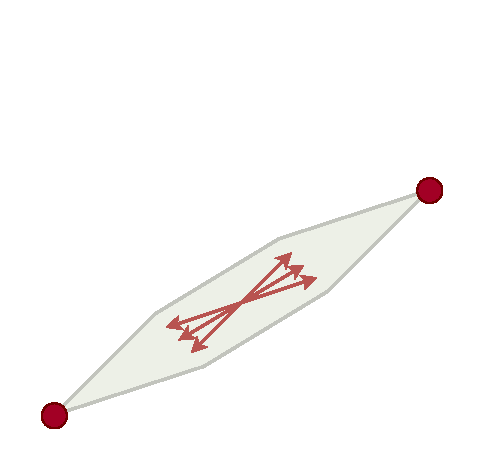
\includegraphics[trim={0 0 0 80},clip, width=0.5\linewidth]{img/chapter_2/stinson_algo_fail.pdf}
    
    \caption{Stinson et al.'s randomized vertex enumeration algorithm. This is an example where the generators are very close angle-wise to each other. In this case, the chosen random vertices have a high probability to correspond to the same zonotope vertex (in red). The sampling size must be increased to avoid this effect.}
    \label{fig:stinson_fail}
\end{figure}

\paragraph*{Skuric et al.'s iterative convex hull method (ICH) \cite{skuricOnLineFeasibleWrench2022}.}
Recently, a novel approximation of a polytope surfaces has been proposed in Skuric et al. \cite{skuricOnLineFeasibleWrench2022}. The following figures \ref{fig:ich_method} summarize this method. For a zonotope $\Zono(n,m)$ in $\IRn$, this algorithm begins with a selection of $n$ direction vectors in $\IRn$ then compute the intersection of their associated line with the zonotope itself. While this requires to describe a set of bounding hyperplanes of $\Zono$, (which we do not have when using a generator matrix representation), it can be leveraged by working in the $m$-cube whose bounding hyperplanes can be enumerated easily. Indeed, the previously generated line in $\IRn$ is also a line in $\IRm$, so there remains to intersect it with the $m$-cube to return two vectors whose projection will map onto the line intersection with the zonotope bounding hyperplanes. Once all intersection points found, compute their convex hull and describe their bounding hyperplanes. Redo the intersection process from the line whose direction are the hyperplane normals. After multiple iterations, the algorithm stops when the produced points in $\IRm$ are sufficiently close, up to some tolerance, to a zonotope vertex.
A Python implementation is available and described in \cite{skuricPycapacityRealtimeTaskspace2023}.

\begin{figure}[!htb]
    \captionsetup{justification=centering}
    \centering
    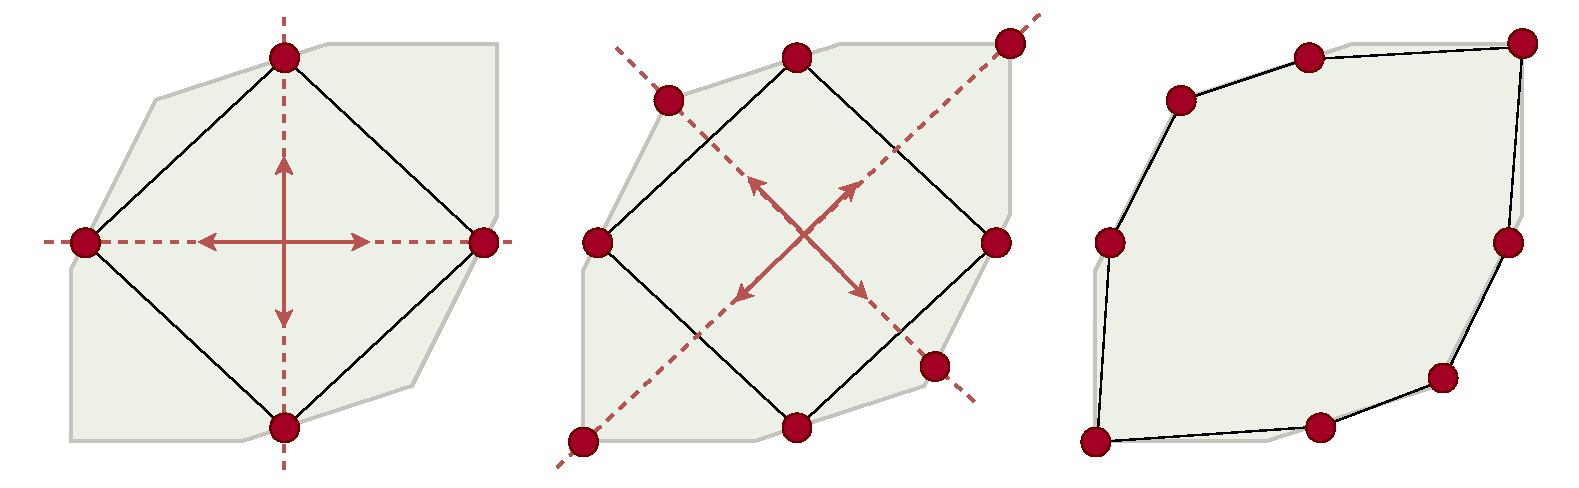
\includegraphics[trim={0 0 0 0},clip, width=1\linewidth]{img/chapter_2/ich_method.pdf}
    
    \caption{In black: the zonotope returned by the Iterative Convex Hull method. To the left: choose $n=2$ vectors in general position, and compute by a linear program its intersection with the given zonotope. Compute the faces of the newly created polytope. At the middle: for each new face, consider the line directed by its normal and intersect it with $\Zono$ using a linear program. To the right: repeat the process until the distance between a created face and the zonotope is less than a specified tolerance.}
    \label{fig:ich_method}
\end{figure}


To compare the quality of produced vertices from each of these algorithm, a metric should be defined. While there exists a computable distance between sets of points involving the euclidean distance from every point of a set to every point of another set (called \emph{Hausdorff} distance), it is not necessarily a relevant metric. Indeed, Skuric et al's method returns a sensible amount of point which are close to the surface of the zonotope, much more than the expected number of vertices. Since it is the global shape of the zonotope which interests us, comparing the relative distance of returned points and the exact vertices would not give a strong information on whether or not the zonotope's surface is well approximated. Instead, we shall use the \emph{Jaccard index}, also called the Jaccard similarity coefficient. It is defined for any two sets $A$ and $B$ as
$$J(A, B) = \frac{\text{Vol}(A\cap B)}{\text{Vol}(A\cup B)}$$
where $\text{Vol}$ denotes the volume. 
If two sets are superposed, then the Jaccard index equals $1$.
For both presented algorithms, the returning points are \emph{on} the surface of the given zonotope, so that the intersection and union are computed easily.

The two next tables summarize both algorithm computation time for $4$-dimensional zonotopes with either $m=15$ or $m=20$ generators. Table \ref{tab:approx_vertex_set_stinson} shows results for Stinson et al.'s algorithm and table \ref{tab:approx_vertex_set_ich} for Skuric et al's. All computations have been performed using the same setup as the previous time benchmark in subsection \ref{subsec:benchmark_results}.
% \subsection{Benchmark results}
\begin{table}[!ht]
    \centering
    \begin{tabular}{|c|c|c|c|c|}
    \hline
    $(n,m)$ & \makecell{Number of \\ samples} & \makecell{Computation \\ time} & \makecell{Number found points \\ / exact number of vertices} & \makecell{Jaccard \\ index} \\
    \hline
    \hline

    % $(2, 10)$ & $<0.01$ & $<0.01$ & $<0.01$ & $<0.01$ \\
    % \hline
    \multirow{ 4}{*}{$(4,15)$} & $10$ & $<0.01$ & $0.41\pm 0.03$ & $0.98\pm 0.01$  \\
    \cline{2-5}
     & $100$ & $<0.01$ & $0.67\pm 0.05$ & $\mathbf{1.00\pm 0.00}$  \\
     \cline{2-5}
     & $1000$ & $0.05\pm 0.00$ & $0.83\pm 0.02$ & $\mathbf{1.00\pm 0.00}$ \\
    \cline{2-5}
     & $10000$ & $0.30\pm 0.01$ & $0.93\pm 0.01$ & $\mathbf{1.00\pm 0.00}$ \\
    % \cline{2-4}
    \hline
    \multirow{ 4}{*}{$(4,20)$} & $10$ & $<0.01$ & $0.28\pm 0.01$ & $0.97\pm 0.00$ \\
    \cline{2-5}
     & $100$ & $0.02\pm 0.00$ & $0.56\pm 0.03$ & $\mathbf{1.00\pm 0.00}$ \\
    \cline{2-5}
     & $1000$ & $0.08\pm 0.00$ & $0.78\pm 0.03$ & $\mathbf{1.00\pm 0.00}$ \\
    \cline{2-5}
     & $10000$ & $0.39\pm 0.02$ & $0.89\pm 0.01$ & $\mathbf{1.00\pm 0.00}$ \\
    \hline
    \end{tabular}
    \caption{Stinson's et al randomized algorithm. $10$ randomly generated $4$-dimensional zonotopes with $m$ generators are computed for each line. The number of samples column correspond to the number of vertices randomly drawn at each iteration. Computation time are in seconds.}
    \label{tab:approx_vertex_set_stinson}
\end{table}

\begin{table}[!ht]
    \centering
    \begin{tabular}{|c|c|c|c|c|}
    \hline
    $(n,m)$ & Tolerance & \makecell{Computation \\ time} & \makecell{Number found points \\ / exact number of vertices} & \makecell{Jaccard \\ index} \\
    \hline
    \hline

    % $(2, 10)$ & $<0.01$ & $<0.01$ & $<0.01$ & $<0.01$ \\
    % \hline
    \multirow{ 4}{*}{$(4,15)$} & $1$ & $0.03\pm 0.01$ & $0.03\pm 0.01$ & $0.56\pm 0.05$  \\
    \cline{2-5}
    & $0.1$ & $0.29\pm 0.02$ & $0.72\pm 0.10$ & $0.98\pm 0.00$ \\
    \cline{2-5}
    & $0.01$ & $0.39\pm 0.01$ & $1.94\pm 0
    .6$ & $\mathbf{1.00\pm 0.00}$\\
    \cline{2-5}
    & $0.001$ & $0.39\pm 0.02$ & $2.12\pm 0.04$ & $\mathbf{1.00\pm 0.00}$ \\
    \hline
    \multirow{ 4}{*}{$(4,20)$}& $1$ & $0.06\pm 0.01$ & $0.03\pm 0.01$ & $0.68\pm 0.05$ \\
    \cline{2-5}
    & $0.1$ & $0.54\pm 0.03$ & $0.61\pm 0.05$ & $0.99\pm 0.00$ \\
    \cline{2-5}
    & $0.01$ & $0.64\pm 0.04$ & $1.36\pm 0.07$ & $\mathbf{1.00\pm 0.00}$ \\
    \cline{2-5}
    & $0.001$ & $0.62\pm 0.04$ & $1.37\pm 0.07$ & $\mathbf{1.00\pm 0.00}$ \\
    \hline
    \end{tabular}
    \caption{Skuric et al ICH algorithm. $10$ randomly generated $4$-dimensional zonotopes with $m$ generators are computed for each line. The tolerance refers to how close should be a computed point from the zonotope surface. Computation time are in seconds.}
    \label{tab:approx_vertex_set_ich}
\end{table}

These tables confirm that both algorithms can produce a set of points assuring a similar shape to a given zonotope. Stinson's et al produces such a set very fastly compared to exact algorithms, and with a number of required points much less than the exact amount. However, Skuric et al's method requires a to set a low tolerance in order to ensure its produced points are close to the zonotope surface, inducing longer computation time related to a higher amount of generated points. 

While results concerning exact and approximation algorithms are related to the surface description of a zonotope, they are strictly different problems. This section showed that in our context of describing the shape of the torque feasible set, an exact enumeration algorithm should \textbf{not} be used when considering a large amount of muscles. However, working with exact algorithms allowed to have more insights upon the geometric process occuring when describing the projection of a  tension set when it is modelized as an orthotope. This understanding is the key to generalize the projection process for any convex shape for $\mathcal{T}$, and is the focus of the next chapter \ref{chapter:3}.

\section{Conclusion}
\label{conclusion_zonotope_enum_algorithm}
In this chapter, we focused on computing explicitely the torque feasible set $\{ -L^T\mathbf{t} - \mathbf{G}\in \IRn \mid \mathbf{t}\in\mathcal{T}\subset \IRm \}$ assuming that $\mathcal{T}$ was shaped as an orthotope, and without loss of generality as a $m$-dimensional cube. The produced set is thus a zonotope, which can be described through various representations including a set of  vertices. However, in our case the torque feasible set is associated to the matrix $-L^T$, which do not directly describe the global shape of its associated zonotope. We then proposed an efficient algorithm, called EdgeEnum, to compute the exact vertices of a zonotope based on its edge enumeration. It was compared theoretically in time and space complexity against various state-of-the-art zonotope enumeration algorithms, to show that we created a theoretically performant algorithm for worst case scenarii, \emph{i.e.} when the number of columns of $-L^T$ is large compared to its number of rows. In simpler terms, when $n\ll m$. 

However, in practice our algorithm can not be performant due to the unavoidable combinatorial amount of vertices to enumerate. A time benchmark has been performed to show that EdgeEnum can be faster than state-of-the-art algorithms when $n\geq 6$ and $m> 10$, but still requires a considerable amount of time in our context. Nevertheless, the next paragraphs summarize the benefits and limits of using an edge-based algorithm.

\subsection{Strengths of EdgeEnum}
EdgeEnum showed several advantages from its creation process to its implementation.

\paragraph*{Easy to implement.} EdgeEnum is straight-forward to implement.
While a recursive version is possible (and implemented in its associated Python package), we prefered to show an implementation based on an iterative construction of edges of a $m$-cube. This is to emphasize readibility as well as the geometric intuition. The only requirement needed for an implementation in any language is the availability of the convex hull operation, which fortunately is already implemented in R, MatLAB, Python and Julia which are common scientific programming languages.

\paragraph*{Parallelism.} A strong advantage of EdgeEnum compared to recent development such as Gu et al. \cite{guCounterfactualIdentificationLatent2022} algorithm is the possibility to parallelize \emph{easily} EdgeEnum. This step occurs during the grouping process, in which all current edges during an iteration are separated into groups according to their directions: applying the convex hull on a group of edge do not require the resulting convex hull of another group. Our Python implementation offers the parallel and non-parallel version of EdgeEnum.

\paragraph*{Theoretical efficiency when $n$ is fixed.} Theorems \ref{th:time_complexity_n_fixed} and \ref{th:space_complexity_n_fixed} showed that our algorithm was polynomialy bounded in the input and output sizes both in time and space complexity. This is fundamental as it qualifies EdgeEnum as an efficient algorithm in time and space. 

\paragraph*{Faster than the state-of-the-art for large $m$ and $n>6$.} While related to the theoretical notion of efficiency, the numerical time benchmarks show that in practice EdgeEnum is indeed faster than state-of-the-arts algorithms when dealing with a zonotope of generator matrix in $\IRnm$. It should be noted that for $n=2$, our algorithm can never be better than Gu et al.'s algorithm, since they reach almost optimality in this specific case.

\paragraph*{EdgeEnum handles degeneracy.} Degeneracy of a zonotope describes if its generators are in general position or not. If they are, the zonotope is not degenerate. The only condition to handle it is the ability of the convex hull operation to return multiple points which are located at the same position. In this case, the convex hull time complexity is not $O(n\log h)$ where $n$ is the number of points and $h$ the number of points on the convex hull: it is instead $O(n\log n)$ on average, using an algorithm like \emph{QuickHull} \cite{barberQuickhullAlgorithmConvex1996}. When applying this new bound into our computed theoretical complexities, this actually does not modify the returning result. However, our computed complexities becomes \emph{average} bounds, and not worst-case bounds. 

However, there are several drawbacks as we shall describe it in the paragraphs.

\subsection{Limits}
We can state that in our case, there are three types of limits related to theoretical algorithmic results, extension of our method to polytopes, and to our context thesis of grasping knowledge about a zonotope surface.

\paragraph*{Non-compactness.} An algorithm is \emph{compact} if its space complexity is polynomially bounded by the input size only \cite{fukudaZonotopeConstructionMinkowski2004a}.
While our new approach is polynomialy bounded in time and space for $n$ fixed, it requires to store all edges found in each iteration.
Our algorithm does not have the property of \emph{compactness}, which means that its space complexity is polynomially bounded by the input size only \cite{fukudaZonotopeConstructionMinkowski2004a}. Indeed, the input size is the generator matrix, which is of size $nm$, and even for $n$ fixed, since the space complexity is in this case $O(m^{n+2})$, it is not bounded by some polynomial $(nm)^{\alpha}$, for $\alpha$ a positive real number. In other words, our algorithm is not able to stream all edges once found, since an edge can be rejected in a next iteration.

As explained by Ferrez et al. \cite{ferrezSolvingFixedRank2005a}, our algorithm lies in the \emph{incremental} strategy category. This means that the edge enumeration problem is solved inductively, by maintaining a list of edges at a certain state and the memory requirement is a critical disadvantage of this kind of approach. So the time efficiency of our algorithm is actually counteracted by its required space.

\paragraph*{Approximation algorithms are better-suited for a fast zonotope surface description.} Even if EdgeEnum remains relevant for practical problems (\cite{guCounterfactualIdentificationLatent2022}, \cite{fukudaZonotopeConstructionMinkowski2004a}, \cite{guibasZonotopesBoundingVolumes}), the description of a zonotope surface is not necessary one of them. Section \ref{sec:approximation_of_vertices_zonotope} showed that there exist algorithms which are sufficiently performant in time to find points on a zonotope surface and whose convex hull is sufficiently close to what should be expected (in volume).

\paragraph*{EdgeEnum does not (always) extend to the vertex enumeration of zonotope sections.} While we showed results concerning the torque feasible set, our main interest as always been the force feasible set \emph{i.e.} a section of a zonotope. If $p$ the dimension of this section equals $n-1$, then it is possible to construct some vertices of the polytope resulting from this section (\emph{cf.} figure \ref{fig:zonotope_section_2D_example}). If the affine subspace sectionning the zonotope is sufficiently in general position (\emph{i.e.} it does not cross any vertices of the zonotope), then it is even possible to enumerate all of its vertices. However, in our context we usually have the force feasible set described in $3D$, the torque space in $7D$ and the tension space in $mD$ for $m\geq 7$, so it is not possible to return all vertices. This is mainly due to the fact the polytope vertices are produced from intersecting this affine space with higher dimensional faces of the zonotope, and not necessarily \emph{only} edges.

\begin{figure}[!htb]
    \captionsetup{justification=centering}
    \centering
    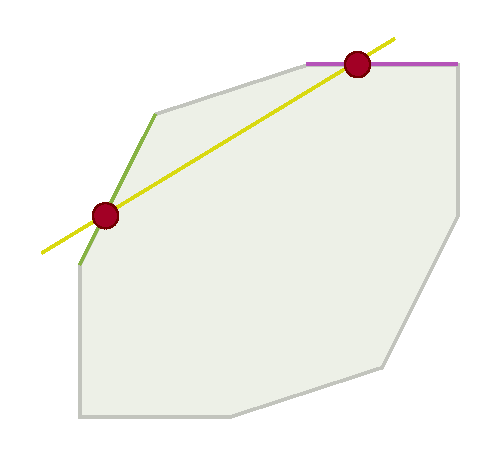
\includegraphics[trim={0 0 0 0},clip, width=0.4\linewidth]{img/chapter_2/polytope_section_zono.pdf}
    \caption{In yellow: an affine subspace $L$ of dimension $1$ which do not intersect zonotope vertices. In this case, and only because $1 = n-1$ with $n=2$ the dimension of the zonotope, it is possible to construct the vertices of this zonotope section by intersecting $L$ with crossing edges.}
    \label{fig:zonotope_section_2D_example}
\end{figure}


\subsection{On the cubic representation of the tension set}

Our novel algorithm is theoretically relevant in the vertex enumeration subfield of Computational Geometry. It sheds new lights onto enumeration techniques. To our knowledge, this is the first time an algorithm uses cube edges combinatorics in order to retrieve vertices. It can be assumed that edges are not necessarily treated as a subject of interest due to their amount (the total number of $m$-cube edges is always much larger than its number of vertices).

In practice, the number of zonotope vertices combinatorially explodes with its number of generators, making \emph{any} enumeration algorithm inefficient in regard to the time computation. In section \ref{sec:approximation_of_vertices_zonotope}, approximations of the zonotope surface have been considered in order to decrease much further the computation time and leveraging the number of points required to describe the zonotope surface. These approximations are relevant in this thesis context: to reconstruct a musculoskeletal model whose torque feasible sets fit given maximal torque capacities in various postures, we must be able to generate in silico a large amout of torque feasible sets and compare them.

However, whether are not approximations or exact algorithms are used, it was underlyingly hypothesized that the tension set has a cubic shape. Biomechanically, this means that all muscles produce their maximum tensions at the same time. In the next chapter, we do not assume this and we diligently focus on the force feasible set shape, for any possible tension set. The creation process of EdgeEnum is a first step in this direction: we described the global shape of the torque feasible set by navigating between the tension set and its projection onto the torque space. In a more general manner, the shape of the tension set and its projection (followed or not by an intersection) are strongly linked. They are even \emph{inextricable}, and the major results of the next chapter serve as argumenting on why does the shape of the tension set does not strictly matter when a large number of muscles is considered. Surprisingly, the understanding of these results led to a novel approximation of \emph{any} projected force feasible set, and a deeper understanding of muscle activation interactions.